% vim:spell spelllang=en:
\documentclass[a4paper,11pt]{article}
\usepackage[utf8]{inputenc}
%\usepackage{fullpage}
\usepackage{listings}
\usepackage{color}
\usepackage{url}
\usepackage{alltt}
\usepackage{multicol}
\usepackage{fancyhdr}
\usepackage{amsmath}
\usepackage{bussproofs}
\usepackage{comment}
\usepackage{inconsolata}
\usepackage{graphicx}

\usepackage{hyperref}
\definecolor{darkgreen}{rgb}{0.0,0.5,0.0}
\hypersetup{colorlinks=true,citecolor=darkgreen}

\renewcommand{\familydefault}{\sfdefault} % change to sans serif font

\newcommand{\seq}{\vdash}	% the sequent sign
\newcommand{\impl}{\supset} %logical connectives: implies, not, and, or
\renewcommand{\lnot}{\neg}
\renewcommand{\land}{\wedge}
\renewcommand{\lor}{\vee}
\newcommand{\sklabel}[2]{\langle#1\rangle^{#2}}

%Commands for constructing proof trees with bussproofs. See the chapter on the LK system for examples.
\newcommand{\UnaryInfCm}[1]{\UnaryInfC{$#1$}}
\newcommand{\BinaryInfCm}[1]{\BinaryInfC{$#1$}}
\newcommand{\RightLabelm}[1]{\RightLabel{$#1$}}
\newcommand{\AxiomCm}[1]{\AxiomC{$#1$}}

% Normal text in math mode ("math text")
\newcommand{\mt}[1]{\textnormal{#1}}
% CLI-style names,words,... within normal text
\newcommand{\cli}[1]{{\ttfamily {#1}}}

\usepackage[draft]{fixme}
\fxsetup{inline,nomargin,marginclue,theme=color,index}

\lstset{
  basicstyle=\small\ttfamily,
  breaklines=true,
%
  frame=leftline,
  framesep=1ex,
  framerule=1ex,
  rulecolor={\color[rgb]{0.8,0.8,0.8}},
%
  inputencoding=utf8,
  extendedchars=true,
  columns=flexible,
  morecomment=[l][\bfseries]{gapt> },
  literate=%
    % FIXME: figure out why the Unicode symbols "eat" their trailing spaces
    {⊥}{{\ensuremath{\bot}} }1%
    {⊤}{{\ensuremath{\top}} }1%
    {∧}{{\ensuremath{\land}} }1%
    {⊃}{{\ensuremath{\impl}} }1%
    {∨}{{\ensuremath{\lor}} }1%
    {¬}{{\ensuremath{\neg}} }1%
    {→}{{\ensuremath{\rightarrow}} }1%
    {∀}{{\ensuremath{\forall}}}1%
    {∃}{{\ensuremath{\exists}}}1%
    {ι}{{\ensuremath{\iota}}}1%
    {α}{{\ensuremath{\alpha}}}1%
    {β}{{\ensuremath{\beta}}}1%
    {τ}{{\ensuremath{\tau}}}1%
    {λ}{{\ensuremath{\lambda}}}1%
    {∈}{{\ensuremath{\in}}}1%
  }

% = clilisting environment
%
% This environment contains CLI interactions which are automatically evaluated
% using "sbt evalUserManual".
%
% Usage:
%
% \begin{clilisting}
% gapt> true
% res1: Boolean = true
% \end{clilisting}
%
% \begin{clilisting}[someCondition]
% gapt> this will only be executed if someCondition returns true
% \end{clilisting}
%
\lstnewenvironment{clilisting}[1][]{}{}

\lstdefinelanguage{scala}{
  morekeywords={abstract,case,catch,class,def,%
    do,else,extends,false,final,finally,%
    for,if,implicit,import,match,mixin,%
    new,null,object,override,package,%
    private,protected,requires,return,sealed,%
    super,this,throw,trait,true,try,%
    type,val,var,while,with,yield},
  otherkeywords={=>,<-,<\%,<:,>:,\#,@},
  sensitive=true,
  showstringspaces=false,
  morecomment=[l]{//},
  morecomment=[n]{/*}{*/},
  morestring=[b]",
  morestring=[b]',
  morestring=[b]"""
}

\lstnewenvironment{tacticslisting}[1][]{\lstset{language=scala}}{}
\lstnewenvironment{tacticsoutput}{}{}

\setlength{\parindent}{0pt}
\setlength{\parskip}{4pt}
\setlength{\headheight}{14pt}
\setlength{\oddsidemargin}{1pt}
\setlength{\textwidth}{450pt}
%\setlength{\textheight}{600pt}

\pagestyle{fancy}
\lhead{GAPT -- User Manual}
\chead{}
\rhead{}

\begin{document}
\begin{titlepage}
\begin{center}

\hrule

\vspace*{20mm}

{\Huge GAPT}

\vspace*{5mm}

{\huge General Architecture for Proof Theory}

\vspace*{20mm}

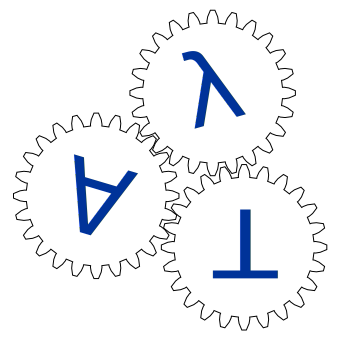
\includegraphics[keepaspectratio,width=5cm]{logo}

\vspace*{20mm}

{\Huge User manual}

\vspace*{10mm}
{\Large Version 2.2-SNAPSHOT}
\vspace*{10mm}

{\Large \today}

\vspace*{20mm}

\hrule
\end{center}

\end{titlepage}

\listoffixmes

\tableofcontents
\vfill
\pagebreak

\section{Introduction}

GAPT is a generic architecture for proof transformations implemented in Scala.

The focus of GAPT are proof transformations (in contrast to proof assistants,
whose focus is proof formalization, and automated deduction systems, whose focus
is proof search). GAPT is used from a shell that provides access to the functionality
in the system in a way that is inspired by computer algebra systems: the basic
objects are formulas and (different kinds of) proofs which can be modified
by calling GAPT commands from the command line. In addition, there
is a graphical user interface that allows the user to view (and—to a certain extent—
modify) proofs in a flexible and visually appealing way.

The current functionality of GAPT includes data structures for formulas,
sequents, resolution proofs, sequent calculus proofs, expansion tree proofs and
algorithms for e.g.\ unification, proof Skolemization, cut-elimination, cut
elimination by resolution~\cite{Baaz00CutElimination},
cut-introduction~\cite{Hetzl2012}, etc.

\section{Download and execution}

There are three ways you can obtain GAPT:

\begin{enumerate}

\item {\bfseries The recommended way:}  You can download a package of the current
version of GAPT at~\url{https://logic.at/gapt/}.  After extracting
the \texttt{tar.gz}-file, you will find a shell script \texttt{gapt.sh}.

Running this script will start the command line interface of GAPT:
\begin{lstlisting}
./gapt.sh
\end{lstlisting}

\item If you are adventurous, you can also download an unstable development
  version from github:
\begin{lstlisting}
git clone https://github.com/gapt/gapt
cd gapt
sbt console
\end{lstlisting}

\item If you like GAPT and want to use it as a library in your Scala project,
  it is available as a Maven artifact on JCenter.  All you need to do is add
  two lines to your \verb,build.sbt,:
\begin{lstlisting}
resolvers += Resolver.jcenterRepo
libraryDependencies += "at.logic.gapt" %% "gapt" % "2.1"
\end{lstlisting}

\end{enumerate}

The command line interface of GAPT is an interactive Scala shell.  This means
that all functionality of Scala is available to you.  In particular it is easy
to write Scala scripts that use the functionality of GAPT.

You don't need to know anything about Scala to try out the examples in this
manual, but if you do want to learn more about Scala we recommend the book
``Programming in Scala''~\cite{odersky2008programming}.

Interactions with the Scala shell are typeset in the following way:
\begin{clilisting}
gapt> println("Hello, world!")
Hello, world!

\end{clilisting}
Here, {\bfseries \cli{println("Hello, world!")}} is the user input, and \texttt{Hello,
world!} is the output from the Scala shell.

If you want to consult the in-depth API documentation of a function, you can
use the \cli{help} command:
\begin{clilisting}
gapt> help(containsQuantifierOnLogicalLevel)

\end{clilisting}

\subsection{System requirements}
\label{sec:sysreq}

To run GAPT you need to have Java 7 (or higher) installed.

GAPT contains interfaces to the following automated reasoning systems. Installing
them is optional. If GAPT does not find the executables in the path, the
functionality of these systems will not be available.

\begin{itemize}
\item Prover9 (\url{http://www.cs.unm.edu/~mccune/mace4/download/}) - make sure
  the commands \texttt{prover9} and \texttt{prooftrans} are available.
\item E theorem prover (\url{http://eprover.org/})
\item Vampire 4.0 (\url{http://www.vprover.org/})
\item SPASS (\url{http://www.spass-prover.org/})
\item LeanCoP (\url{http://leancop.de/})
\item Metis (\url{http://www.gilith.com/software/metis/})
\item VeriT (\url{http://www.verit-solver.org/})
\item Z3 (\url{https://github.com/Z3Prover/z3})
\item MiniSAT (\url{http://minisat.se/})
\item Glucose (\url{http://www.labri.fr/perso/lsimon/glucose/})
\item PicoSAT (\url{http://fmv.jku.at/picosat/})
\item Sat4J (\url{http://sat4j.org/})
\item OpenWBO (\url{http://sat.inesc-id.pt/open-wbo/})
\item CVC4 (\url{http://cvc4.cs.nyu.edu/web/})
\end{itemize}

\section{Data structures}

\subsection{Expressions and formulas}

Formulas, terms, and other expressions are are represented as lambda terms in a
simple type theory with many base sorts.  The standard base sorts are $o$ for
Boolean values, and $\iota$ for individuals.  Terms and formulas of first-order
logic and higher-order logic are hence encoded as lambda terms, these
form regular subsets of the lambda expression.

There are two ways of entering expressions: you can parse them or construct them
manually.
\subsubsection{Formula parsing}
Here is an example of parsing a first-order formula:
\begin{clilisting}
gapt> val F = fof"!x (P(x,f(x)) -> ?y P(x,y))"
F: at.logic.gapt.expr.FOLFormula = ∀x (P(x, f(x)) ⊃ ∃y P(x, y))

\end{clilisting}

Every kind of expression that GAPT supports can be parsed by writing \verb!<prefix>"<string>"!.
The prefix indicates the Scala type of the expression. The following prefixes are available:

\begin{tabular}{r l}
\cli{le} & lambda expression \\
\cli{hof} & higher-order formula \\
\cli{hoa} & higher-order atom \\
\cli{hov} & higher-order variable \\
\cli{hoc} & higher-order constant \\
\cli{foe} & first-order expression \\
\cli{fof} & first-order formula \\
\cli{fot} & first-order term \\
\cli{foa} & first-order atom \\
\cli{fov} & first-order variable \\
\cli{foc} & first-order constant
\end{tabular}

This parser supports Scala string interpolation. For example, you can do:
\begin{clilisting}
gapt> val t = fot"f(f(x))"
t: at.logic.gapt.expr.FOLTerm = f(f(x))

gapt> val G = fof"!x (P(x,$t) -> ?y P(x,y))"
G: at.logic.gapt.expr.FOLFormula = ∀x (P(x, f(f(x))) ⊃ ∃y P(x, y))

\end{clilisting}


The input language has full type inference, and the formula
prefixes make sure that the expression is of type $o$ (Boolean).  If no
particular type is required, we default to $\iota$:
\begin{clilisting}
gapt> hof"!x?y!z x(z) = y(y(z))"
res2: at.logic.gapt.expr.HOLFormula = ∀x ∃y ∀z x(z) = y(y(z))

\end{clilisting}

So far we have only used the ASCII-safe part of the syntax, however Unicode
input is of course supported as well---you can paste any of the output right
back in:
\begin{clilisting}
gapt> hof"∀x ∃y ∀z x(z) = y(y(z))"
res3: at.logic.gapt.expr.HOLFormula = ∀x ∃y ∀z x(z) = y(y(z))

\end{clilisting}

Here is a summary of the available syntax (there are usually multiple variants
of each construct, these are separated by commas here):

\begin{tabular}{r l}
\cli{x1}, \cli{uvw} & variables (need to start with \cli{u-z} or \cli{U-Z}, or be bound) \\
\cli{c}, \cli{theorem} & constants \\
\cli{f(x,c)}, \cli{f(x)(c)}, \cli{f x c} & function application \\
\cli{\textbackslash x f(x)}, \cli{$\lambda$x f(x)}, \cli{\^{}x f(x)} & lambda abstraction \\
\cli{!x p(x)}, \cli{!(x:i) p(x)}, \cli{$\forall$x p(x)} & universal quantification \\
\cli{?x p(x)}, \cli{?(x:i) p(x)}, \cli{$\exists$x p(x)} & existential quantification \\
\cli{-p}, \cli{$\neg$ p} & negation \\
\cli{p \& q}, \cli{p $\land$ q} & conjunction \\
\cli{p | q}, \cli{p $\lor$ q} & disjunction \\
\cli{p -> q}, \cli{p $\impl$ q} & implication \\
\cli{p <-> q} & equivalence (this is the same as \cli{p $\impl$ q $\land$ q $\impl$ p}) \\
\cli{p = q}, \cli{p = q = r} & equality \\
\cli{p != q} & disequality \\
\cli{p < q <= r > s >= t} & various infix relations \\
\cli{a*b/c + d - e} & infix operators \\
\cli{f: i>i>o} & type annotation
\end{tabular}

\subsubsection{Constructing formulas manually}
Every kind of expression that exists in GAPT can be constructed manually. For instance, you can define variables
and constants like this:
\begin{clilisting}
gapt> val x = FOLVar("x")
x: at.logic.gapt.expr.FOLVar = x

gapt> val P = Const("P", Ti -> To)
P: at.logic.gapt.expr.Const = P:i>o

\end{clilisting}
\cli{Var} and \cli{Const} require you to supply types, whereas \cli{FOLVar} and
\cli{FOLConst} automatically have type $\iota$. Terms and atomic formulas are constructed
similarly:
\begin{clilisting}
gapt> val x = FOLVar("x")
x: at.logic.gapt.expr.FOLVar = x

gapt> val fx = FOLFunction("f",x)
fx: at.logic.gapt.expr.FOLTerm = f(x)

gapt> val Pfx = FOLAtom("P", fx)
Pfx: at.logic.gapt.expr.FOLAtom = P(f(x)): o

\end{clilisting}

On the formulas themselves, there are operators for the various Boolean connectives:

\begin{tabular}{r l}
 \cli{-A} & $\neg A$\\
 \cli{A \& B} & $A \wedge B$\\
 \cli{A | B} & $A \vee B$\\
 \cli{A --> B} & $A \supset B$\\
 \cli{A <-> B} & $A \leftrightarrow B$
\end{tabular}
 
\begin{clilisting}
gapt> val A = FOLAtom("A")
A: at.logic.gapt.expr.FOLAtom = A:o

gapt> val B = FOLAtom("B")
B: at.logic.gapt.expr.FOLAtom = B:o

gapt> val C = FOLAtom("C")
C: at.logic.gapt.expr.FOLAtom = C:o

gapt> (A & B) --> C
res4: at.logic.gapt.expr.FOLFormula = A ∧ B ⊃ C

\end{clilisting}

\subsubsection{Predefined formulas}

A collection of formula sequences can be found in the file \cli{examples/FormulaSequences.scala}.
You can generate instances of these formula sequences by entering for example:
\begin{clilisting}
gapt> val f = BussTautology( 5 )
f: at.logic.gapt.proofs.HOLSequent =
((c_1 ∨ d_1) ∧ (c_2 ∨ d_2) ∧ (c_3 ∨ d_3) ∧ (c_4 ∨ d_4) ⊃ c_5) ∨
  ((c_1 ∨ d_1) ∧ (c_2 ∨ d_2) ∧ (c_3 ∨ d_3) ∧ (c_4 ∨ d_4) ⊃ d_5),
((c_1 ∨ d_1) ∧ (c_2 ∨ d_2) ∧ (c_3 ∨ d_3) ⊃ c_4) ∨
  ((c_1 ∨ d_1) ∧ (c_2 ∨ d_2) ∧ (c_3 ∨ d_3) ⊃ d_4),
((c_1 ∨ d_1) ∧ (c_2 ∨ d_2) ⊃ c_3) ∨ ((c_1 ∨ d_1) ∧ (c_2 ∨ d_2) ⊃ d_3),
(c_1 ∨ d_1 ⊃ c_2) ∨ (c_1 ∨ d_1 ⊃ d_2),
c_1 ∨ d_1
:-
c_5:o,
d_5:o

\end{clilisting}

\subsection{Sequents}
Sequents are an important data structure in GAPT. A sequent is a pair of lists:
\begin{equation*}
 A_1,...,A_m \vdash B_1,...,B_n
\end{equation*}
The list to the left of the sequent symbol $\vdash$ is called the antecedent, the
one on the right the succedent. Usually, but not always, the elements of the sequences are going to be formulas.

In GAPT, you can create sequents by supplying an antecedent and a succedent:

\begin{clilisting}
gapt> val S1 = Sequent() // the empty sequent
S1: at.logic.gapt.proofs.Sequent[Nothing] =  :-

gapt> val S2 = Sequent(List(1,2), List(3,4)) // a sequent of Ints
S2: at.logic.gapt.proofs.Sequent[Int] = 1, 2 :- 3, 4

gapt> val S3 = Sequent(List(foa"A", foa"B"), List(foa"C", foa"D")) // a sequent of FOL atoms
S3: at.logic.gapt.proofs.Sequent[at.logic.gapt.expr.FOLAtom] = A:o, B:o :- C:o, D:o

\end{clilisting}

Sequents have append operations for both the antecedent and the succedent. In the antecedent,
elements are appended to the left, in the succedent, to the right:

\begin{clilisting}
gapt> val S1 = Sequent(List(foa"B"), List(foa"C"))
S1: at.logic.gapt.proofs.Sequent[at.logic.gapt.expr.FOLAtom] = B:o :- C:o

gapt> val S2 = foa"A" +: S1
S2: at.logic.gapt.proofs.Sequent[at.logic.gapt.expr.FOLAtom] = A:o, B:o :- C:o

gapt> val S3 = S2 :+ foa"D"
S3: at.logic.gapt.proofs.Sequent[at.logic.gapt.expr.FOLAtom] = A:o, B:o :- C:o, D:o

gapt> foa"A" +: foa"B" +: Sequent() :+ foa"C" :+ foa"D"
res5: at.logic.gapt.proofs.Sequent[at.logic.gapt.expr.FOLAtom] = A:o, B:o :- C:o, D:o

\end{clilisting}

You can retrieve elements from a sequent either by accessing the antecedent
or succedent directly ...
\begin{clilisting}
gapt> val S = Sequent(List(foa"A", foa"B"), List(foa"C", foa"D"))
S: at.logic.gapt.proofs.Sequent[at.logic.gapt.expr.FOLAtom] = A:o, B:o :- C:o, D:o

gapt> val b = S.antecedent(1)
b: at.logic.gapt.expr.FOLAtom = B:o

gapt> val c = S.succedent(0)
c: at.logic.gapt.expr.FOLAtom = C:o

\end{clilisting}
... or by using the \cli{SequentIndex} class:

\begin{clilisting}
gapt> val i = Ant(0)
i: at.logic.gapt.proofs.Ant = Ant(0)

gapt> val j = Suc(1)
j: at.logic.gapt.proofs.Suc = Suc(1)

gapt> val a = S(i)
a: at.logic.gapt.expr.FOLAtom = A:o

gapt> val d = S(j)
d: at.logic.gapt.expr.FOLAtom = D:o

\end{clilisting}


\subsection{Proofs}\label{sec:entering_proofs}

There are various possibilities for entering proofs into the system. The most
basic one is a direct top-down proof-construction using the constructors
of the inference rules.

\subsubsection{Top-down proof construction}
We start with the axioms:
%
\begin{clilisting}
gapt> val p1 = LogicalAxiom(fof"A")
p1: at.logic.gapt.proofs.lk.LogicalAxiom =
[p1] A:o :- A:o    (LogicalAxiom(A:o))

gapt> val p2 = LogicalAxiom(fof"B")
p2: at.logic.gapt.proofs.lk.LogicalAxiom =
[p1] B:o :- B:o    (LogicalAxiom(B:o))

\end{clilisting}
%
These are joined by an $\land:\mathrm{right}$-inference. See Appendix~\ref{app:sequent_calculus}
for the formal definition of the sequent calculus used in GAPT.
\begin{clilisting}
gapt> val p3 = AndRightRule( p1, fof"A", p2, fof"B" )
p3: at.logic.gapt.proofs.lk.AndRightRule =
[p3] A:o, B:o :- A ∧ B    (AndRightRule(p1, Suc(0), p2, Suc(0)))
[p2] B:o :- B:o    (LogicalAxiom(B:o))
[p1] A:o :- A:o    (LogicalAxiom(A:o))

\end{clilisting}
%
To finish the proof it remains to apply two $\impl:\mathrm{right}$-inferences:
%
\begin{clilisting}
gapt> val p4 = ImpRightRule( p3, fof"B", fof"A & B" )
p4: at.logic.gapt.proofs.lk.ImpRightRule =
[p4] A:o :- B ⊃ A ∧ B    (ImpRightRule(p3, Ant(1), Suc(0)))
[p3] A:o, B:o :- A ∧ B    (AndRightRule(p1, Suc(0), p2, Suc(0)))
[p2] B:o :- B:o    (LogicalAxiom(B:o))
[p1] A:o :- A:o    (LogicalAxiom(A:o))

gapt> val p5 = ImpRightRule( p4, fof"A", fof"B -> A&B" )
p5: at.logic.gapt.proofs.lk.ImpRightRule =
[p5]  :- A ⊃ B ⊃ A ∧ B    (ImpRightRule(p4, Ant(0), Suc(0)))
[p4] A:o :- B ⊃ A ∧ B    (ImpRightRule(p3, Ant(1), Suc(0)))
[p3] A:o, B:o :- A ∧ B    (AndRightRule(p1, Suc(0), p2, Suc(0)))
[p2] B:o :- B:o    (LogicalAxiom(B:o))
[p1] A:o :- A:o    (LogicalAxiom(A:o))

\end{clilisting}
%
You can now view this proof by typing:
\begin{clilisting}
gapt> prooftool( p5 )

\end{clilisting}

The system comes with a collection of example proof sequences in the file
\cli{examples/ProofSequences.scala} which are generated in the above style.
Have a look at this code for more complicated proof constructions.
You can generate instances of these proof sequences by entering, e.g.,
\begin{clilisting}
gapt> val p = SumExampleProof( 5 )
p: at.logic.gapt.proofs.lk.LKProof =
[p25] ∀x ∀y (P(s(x), y) ⊃ P(x, s(y))),
P(s(s(s(s(s(0))))), 0): o
:-
P(0, s(s(s(s(s(0)))))): o    (ContractionLeftRule(p24, Ant(0), Ant(1)))
[p24] ∀x ∀y (P(s(x), y) ⊃ P(x, s(y))),
∀x ∀y (P(s(x), y) ⊃ P(x, s(y))),
P(s(s(s(s(s(0))))), 0): o
:-
P(0, s(s(s(s(s(0)))))): o    (ForallLeftRule(p23, Ant(0), ∀y (P(s(x), y) ⊃ P(x, s(y))), 0, x))
[p23] ∀y (P(s(0), y) ⊃ P(0, s(y))),
∀x ∀y (P(s(x), y) ⊃ P(x, s(y))),
P(s(s(s(s(s(0))))), 0): o
:-
P(0, s(s(s(s(s(0)))))): o    (ForallLeftRule(p22, Ant(0), P(s(0), y) ⊃ P(0, s(y)), s(s(s(s(0)))), y))
[p22] P(s(0), s(s(s(s(0))))) ⊃ P(0, s(s(s(s(s(0)))))),
∀x ∀y (P(s(x), y) ⊃ P(x, s(y))),
P(s(s(s(s(s(0))))), 0): o
:-
P(0, s(s(s(s(s(0)))))): o    (ImpLeftRule(p20, Suc(0), p21, Ant(0)))
[p21] P(0, s(s(s(s(s(0)))))): o :- P(0...
\end{clilisting}

\subsubsection{Gaptic}

GAPT also contains a tactics language called gaptic.  In contrast to the
top-down construction presented in the last section, gaptic allows a
comfortable bottom-up development of proofs, similar to popular proof
assistants such as Coq, etc.

Gaptic can not be (easily) used in the interactive Scala shell, as it requires
multi-line input.  Gaptic scripts are usually developed as external files:
\begin{tacticslisting}
import at.logic.gapt.expr._
import at.logic.gapt.proofs.{Context, Sequent}
import at.logic.gapt.proofs.gaptic._

object example extends TacticsProof {
  ctx += Context.Sort("i")
  ctx += hoc"P: i>o"
  ctx += hoc"Q: i>o"

  val lemma = Lemma(
    ("a" -> fof"P a") +:
    ("b" -> fof"∀x (P x ⊃ Q x)") +:
    Sequent()
    :+ ("c" -> fof"Q a")
  ) {
    chain("b")
    chain("a")
  }
}
\end{tacticslisting}
\begin{tacticsoutput}
\end{tacticsoutput}

Gaptic proofs start with a declaration of the used base types and constants.
Each proof is then assigned to a Scala variable.  The function
\verb,Lemma(labelledSequent) { tactics... }, constructs a proof using the
gaptic language.  The first argument of \cli{Lemma} is the labelled end
sequent, i.e. the sequent you want to prove in which each formula has a string
label.  The second argument consists of a list of statements, called tactics,
separated by line breaks:

At the moment, there are two ways to execute gaptic scripts:
\begin{enumerate}

  \item From the Scala shell, using the \cli{:load} command.  This command
    evaluates the Scala file, but \emph{not} the code inside the \cli{object}
    declaration.  So we have to explicitly evaluate the proof ourselves.
\begin{lstlisting}
gapt> :load example.scala
gapt> example.lemma
\end{lstlisting}

  \item As a separate SBT project, see
    \url{https://github.com/gapt/gaptic-example} for a template project.  This
approach has the advantage that SBT can automatically run your script whenever
you save it:
\begin{lstlisting}
> ~runMain example
[info] Running example 
[success] Total time: 1 s, completed Apr 5, 2016 11:16:32 AM
1. Waiting for source changes... (press enter to interrupt)
\end{lstlisting}

\end{enumerate}

Let us use gaptic to input a very simple proof.  Our first try might be the
following (we now omit the boilerplate for brevity):
\begin{tacticslisting}
val lemmaEx =
  Lemma(Sequent(
      Seq("a" -> fof"P a", "b" -> fof"!x (P x -> Q x)"),
      Seq("c" -> fof"Q a"))) {
    allL(fot"a")
  }
\end{tacticslisting}
\begin{tacticsoutput}
at.logic.gapt.proofs.gaptic.QedFailureException: Proof not completed. There are still 1 open sub goals:
b_0: P(a) ⊃ Q(a)
a: P(a): o
b: ∀x (P(x) ⊃ Q(x))
:-
c: Q(a): o

  at at.logic.gapt.proofs.gaptic.LemmaMacros$.finishProof(language.scala:45)
  ... 25 elided
\end{tacticsoutput}

As seen above, the currently open goals are shown when the proof is not yet
completed. Upon completion of the proof, the value of \cli{lemmaEx} is the
resulting proof:
\begin{tacticslisting}
val lemmaEx =
  Lemma(Sequent(
      Seq("a" -> fof"P a", "b" -> fof"!x (P x -> Q x)"),
      Seq("c" -> fof" Q a"))) {
    allL(fot"a")
    impL
    trivial
    trivial
  }
\end{tacticslisting}
\begin{tacticsoutput}
\end{tacticsoutput}

Most tactics can be called with or without a label argument. If a tactic is
called with a label, it will be applied to that specific formula, if possible.
Otherwise, the system will attempt to determine a target formula on its own. If
there is no such formula or more than one, the tactic will fail.

We now give a description of a few tactics, you can see the full list in the
API documentation:
\begin{clilisting}
gapt> help(at.logic.gapt.proofs.gaptic.TacticCommands)

\end{clilisting}

The \cli{forget} tactic corresponds to weakening rules in LK. It accepts a list
of labels and removes the formulas with those labels from the current subgoal:
\begin{tacticslisting}
val lemmaEx =
  Lemma(Sequent(
      Seq("a" -> fof"P a", "b" -> fof"!x (P x -> Q x)"),
      Seq("c" -> fof" Q a"))) {
    forget("b")
  }
\end{tacticslisting}
\begin{tacticsoutput}
at.logic.gapt.proofs.gaptic.QedFailureException: Proof not completed. There are still 1 open sub goals:
a: P(a): o
:-
c: Q(a): o

  at at.logic.gapt.proofs.gaptic.LemmaMacros$.finishProof(language.scala:45)
  ... 25 elided
\end{tacticsoutput}

The tactics \cli{axiomLog}, \cli{axiomRefl}, \cli{axiomBot} and \cli{axiomTop}
cover the logical, reflexivity, bottom and top axioms, respectively. The
\cli{trivial} tactic automatically selects the applicable axiom. Also, any
weakening rules required to reach an actual axiom sequent are automatically
applied.

The following example shows the use of the \cli{trivial} tactic to end the proof by a logical axiom:
\begin{tacticslisting}
val axiomEx =
  Lemma(Sequent(Nil,
      Seq("D" -> fof"exists x (P x -> all y P y)"))) {
    exR(fot"c")
    impR
    allR
    exR(fov"y")
    impR
    allR
    trivial
  }
\end{tacticslisting}
\begin{tacticsoutput}
\end{tacticsoutput}

The tactic \cli{eql} covers the left and right equality rules. The tactic takes
as first argument the label of an equality to use from the antecedent. The
second argument is the label of the formula to apply the rule to. Furthermore,
it can be specified if the equality should be used from left to right or vice
versa. Also, a target formula can be specified, if not all occurrences need to
be replaced (in either direction). If neither direction nor a target formula is
specified, the tactic will only work if the direction is unambiguous.

\begin{tacticslisting}
val eqEx = Lemma(Sequent(
    Seq("c" -> fof"P(y) & Q(y)",
        "eq1" -> fof"u = v",
        "eq2" -> fof"y = x",
        "a" -> fof"P(u) -> Q(u)"),
    Seq("b" -> fof"P(x) & Q(x)"))) {
  eql("eq1", "a").yielding(fof"P(v) -> Q(v)")
  eql("eq1", "a").yielding(fof"P(v) -> Q(u)")
  eql("eq2", "b").fromRightToLeft
  trivial
}
\end{tacticslisting}
\begin{tacticsoutput}
\end{tacticsoutput}

The tactics for the weak quantifiers are \cli{allL} and \cli{exR}. They are
called with the list of terms to instantiate the quantified formula with. One
call of \cli{allL} or \cli{exR} can instantiate any number of quantifiers in a
formula. The tactics for the strong quantifiers are \cli{allR} and \cli{exL}.
They are optionally called with the variable that should be used as an
eigenvariable. If no eigenvariable is provided, a fresh variable will
automatically be generated. The weak quantifier formulas are kept in the
sequent after instantiations while the strong quantifier formulas are
automatically removed.
\begin{tacticslisting}
val quantEx = Lemma(Sequent(
    Seq("D" -> fof"(all x (P(x) & (exists y -P(y))))"),
    Nil)) {
  allL(fot"c")
  andL
  exL(fov"y_0")
  negL
  allL(fot"y_0")
  andL
  exL(fov"y_1")
  negL
  axiomLog
}
\end{tacticslisting}
\begin{tacticsoutput}
\end{tacticsoutput}

The implication, negation, disjunction and conjunction rules are covered by the
tactics \cli{impL}, \cli{impR}, \cli{negL}, \cli{negR}, \cli{disL}, \cli{disR},
\cli{conL} and \cli{conR}, respectively. They are similar in the sense that
they take no arguments apart from an optional label to apply the tactic to.
\begin{tacticslisting}
val propEx = Lemma(Sequent(
    Seq("initAnt" -> fof"A -> B"),
    Seq("initSuc" -> fof"(A & B) | -A"))) {
  orR("initSuc")
  negR("initSuc_1")
  andR("initSuc_0")
  trivial
  impL
  trivial
  trivial
}
\end{tacticslisting}
\begin{tacticsoutput}
\end{tacticsoutput}

The \cli{cut} tactic is used to introduce a cut rule. The first argument is the
(unique new) label for the cut formula, the second argument is the cut formula
itself. Both arguments are mandatory. In the case where a non-unique label is
provided the tactic simply fails.
\begin{tacticslisting}
val cutEx = Lemma(Sequent(
    Seq("A" -> fof"A"),
    Seq("C" -> fof"(exists x exists y ( -x=y & f(x)=f(y) ))"))) {
  cut("I1", fof"I(1)")
  cut("I0", fof"I(0)")
}
\end{tacticslisting}
\begin{tacticsoutput}
at.logic.gapt.proofs.gaptic.QedFailureException: Proof not completed. There are still 3 open sub goals:
A: A:o
:-
C: ∃x ∃y (¬x = y ∧ f(x) = f(y))
I1: I(1): o
I0: I(0): o

I0: I(0): o
A: A:o
:-
C: ∃x ∃y (¬x = y ∧ f(x) = f(y))
I1: I(1): o

I1: I(1): o
A: A:o
:-
C: ∃x ∃y (¬x = y ∧ f(x) = f(y))

  at at.logic.gapt.proofs.gaptic.LemmaMacros$.finishProof(language.scala:45)
  ... 25 elided
\end{tacticsoutput}

Using gaptic, we can also create proofs with induction.  For example, let us
prove that concatenation of lists is associative:

\begin{tacticslisting}[nosig]
ctx += Context.Sort("i")

// Define the type of lists.
ctx += Context.InductiveType("list",
  hoc"nil: list",
  hoc"cons: i>list>list")

// Declare a constant denoting concatenation.
// We will axiomatize its definition in the end-sequent.
ctx += hoc"'+': list>list>list"

val catassoc =
  Lemma(
      ("conscat" -> hof"∀x ∀y ∀z cons(x,y)+z = cons(x,y+z)") +:
      ("nilcat" -> hof"∀x nil+x = x") +:
      Sequent()
      :+ ("goal" -> hof"∀x ∀y ∀z x+(y+z) = (x+y)+z")
    ) {
  induction onAll decompose
  rewrite.many ltr "nilcat"; refl
  rewrite.many ltr ("conscat", "IHx_0"); refl
}
\end{tacticslisting}
\begin{tacticsoutput}
\end{tacticsoutput}

\section{Feature walkthrough}

\subsection{SAT solver interface}
%
The following shows an example session, using the Sat4j SAT solver
to verify validity and satisfiability, and query the thus obtained models.
Consider the {\em pigeon hole principle for $(m, n)$, $\mathrm{PHP}_{m,n}$}, which states that if $m$ pigeons
are put into $n$ holes, then there is a hole which contains two pigeons. It is valid
iff $m>n$. $\neg\mathrm{PHP}_{m,n}$ states that when putting $m$ pigeons into $n$ holes, there
is no hole containing two pigeons. This is satisfiable iff $m\leq n$.
\begin{clilisting}
gapt> Sat4j isValid PigeonHolePrinciple(3, 2)
res8: Boolean = true

\end{clilisting}
shows\footnote{In Scala, \cli{Sat4j isValid formula} is syntactic sugar for \cli{Sat4j.isValid(formula)}.} that $\mathrm{PHP}_{3,2}$ is valid, and
\begin{clilisting}
gapt> Sat4j isValid PigeonHolePrinciple(3, 3)
res9: Boolean = false

\end{clilisting}
shows that $\mathrm{PHP}_{3,3}$ is not valid.
Furthermore,
\begin{clilisting}
gapt> val Some(m) = Sat4j solve -PigeonHolePrinciple(3, 3)
m: at.logic.gapt.models.Interpretation =
R(p_1, h_1): o -> false
R(p_1, h_2): o -> false
R(p_1, h_3): o -> true
R(p_2, h_1): o -> true
R(p_2, h_2): o -> false
R(p_2, h_3): o -> false
R(p_3, h_1): o -> false
R(p_3, h_2): o -> true
R(p_3, h_3): o -> false

\end{clilisting}
yields a model of $\neg\mathrm{PHP}_{3,3}$ that can be queried:
\begin{clilisting}
gapt> val p1 = PigeonHolePrinciple.atom(1, 1)
p1: at.logic.gapt.expr.FOLAtom = R(p_1, h_1): o

gapt> val p2 = PigeonHolePrinciple.atom(2, 1)
p2: at.logic.gapt.expr.FOLAtom = R(p_2, h_1): o

gapt> m.interpret(p1) // Is pigeon 1 in hole 1?
res10: Boolean = false

gapt> m.interpret(p2) // Is pigeon 2 in hole 1?
res11: Boolean = true

\end{clilisting}
We can also interpret quantifier-free formulas:
\begin{clilisting}
gapt> m.interpret( And(p1, p2) )
res12: Boolean = false

\end{clilisting}

We can also convert $\neg\mathrm{PHP}_{3,3}$ into DIMACS format:
\begin{clilisting}
gapt> val cnf = structuralCNF(Sequent() :+ PigeonHolePrinciple(3,3)).map(_.conclusion.asInstanceOf[HOLClause])
cnf: scala.collection.immutable.Set[at.logic.gapt.proofs.HOLClause] = Set(R(p_2, h_3): o, R(p_1, h_3): o :- , R(p_3, h_1): o, R(p_1, h_1): o :- , R(p_2, h_1): o, R(p_1, h_1): o :- , R(p_3, h_2): o, R(p_2, h_2): o :- ,  :- R(p_1, h_3): o, R(p_1, h_1): o, R(p_1, h_2): o,  :- R(p_3, h_3): o, R(p_3, h_1): o, R(p_3, h_2): o, R(p_3, h_3): o, R(p_2, h_3): o :- , R(p_3, h_3): o, R(p_1, h_3): o :- , R(p_2, h_2): o, R(p_1, h_2): o :- ,  :- R(p_2, h_3): o, R(p_2, h_1): o, R(p_2, h_2): o, R(p_3, h_1): o, R(p_2, h_1): o :- , R(p_3, h_2): o, R(p_1, h_2): o :- )

gapt> val encoding = new DIMACSEncoding
encoding: at.logic.gapt.formats.dimacs.DIMACSEncoding = DIMACSEncoding()

gapt> writeDIMACS(encoding encodeCNF cnf)
res13: String =
"p cnf 9 12
-1 -2 0
-3 -4 0
-5 -4 0
-6 -7 0
2 4 8 0
9 3 6 0
-9 -1 0
-9 -2 0
-7 -8 0
1 5 7 0
-3 -5 0
-6 -8 0
"

\end{clilisting}

If you want to know which variable in the DIMACS output corresponds to which
atom in GAPT, you can query the \cli{DIMACSEncoding} object:
\begin{clilisting}
gapt> encoding decodeAtom 1
res14: at.logic.gapt.expr.HOLAtom = R(p_2, h_3): o

\end{clilisting}

GAPT also supports other SAT solvers such as MiniSAT or Glucose out of the box:
\begin{clilisting}[MiniSAT.isInstalled]
gapt> MiniSAT isValid PigeonHolePrinciple(3,2)
res15: Boolean = true

\end{clilisting}
\begin{clilisting}[Glucose.isInstalled]
gapt> Glucose isValid PigeonHolePrinciple(3,2)
res16: Boolean = true

\end{clilisting}

If you have another DIMACS-compliant solver installed or want to pass extra
options to the SAT solver, you can pass a custom command to GAPT as well:
\begin{clilisting}[MiniSAT.isInstalled]
gapt> val solver = new ExternalSATSolver("minisat", "-mem-lim=1024")
solver: at.logic.gapt.provers.sat.ExternalSATSolver = ExternalSATSolver("minisat", "-mem-lim=1024")

gapt> solver isValid PigeonHolePrinciple(3,2)
res17: Boolean = true

\end{clilisting}

GAPT can import DRUP proofs from Sat4j, Glucose, and PicoSAT:
\begin{clilisting}
gapt> Sat4j getDrupProof PigeonHolePrinciple(4,3)
res18: Option[at.logic.gapt.proofs.drup.DrupProof] =
Some([derive]  :-
[derive] R(p_3, h_3): o :-
[derive]  :- R(p_4, h_1): o
[derive] R(p_4, h_3): o :- R(p_3, h_1): o, R(p_1, h_1): o
[derive]  :- R(p_2, h_1): o, R(p_4, h_1): o
[derive] R(p_4, h_2): o :- R(p_2, h_1): o
[input] R(p_1, h_2): o, R(p_4, h_2): o :-
[input] R(p_1, h_3): o, R(p_3, h_3): o :-
[input]  :- R(p_3, h_1): o, R(p_3, h_2): o, R(p_3, h_3): o
[input] R(p_2, h_2): o, R(p_3, h_2): o :-
[input] R(p_1, h_1): o, R(p_2, h_1): o :-
[input] R(p_1, h_3): o, R(p_2, h_3): o :-
[input]  :- R(p_1, h_2): o, R(p_1, h_3): o, R(p_1, h_1): o
[input] R(p_3, h_1): o, R(p_2, h_1): o :-
[input] R(p_3, h_1): o, R(p_1, h_1): o :-
[input] R(p_2, h_2): o, R(p_4, h_2): o :-
[input] R(p_2, h_3): o, R(p_4, h_3): o :-
[input] R(p_2, h_3): o, R(p_3, ...
\end{clilisting}

Just as in the first-order prover interface, you can call
\cli{getResolutionProof} and \cli{getLKProof} to get the proofs in the desired
format:
\begin{clilisting}
gapt> Sat4j getLKProof PigeonHolePrinciple(4,3)
res19: Option[at.logic.gapt.proofs.lk.LKProof] =
Some([p392]
:-
(R(p_1, h_1) ∨ R(p_1, h_2) ∨ R(p_1, h_3)) ∧
    (R(p_2, h_1) ∨ R(p_2, h_2) ∨ R(p_2, h_3)) ∧
    (R(p_3, h_1) ∨ R(p_3, h_2) ∨ R(p_3, h_3)) ∧
    (R(p_4, h_1) ∨ R(p_4, h_2) ∨ R(p_4, h_3)) ⊃
  R(p_2, h_1) ∧ R(p_1, h_1) ∨
    (R(p_3, h_1) ∧ R(p_1, h_1) ∨ R(p_3, h_1) ∧ R(p_2, h_1)) ∨
    (R(p_4, h_1) ∧ R(p_1, h_1) ∨
      R(p_4, h_1) ∧ R(p_2, h_1) ∨
      R(p_4, h_1) ∧ R(p_3, h_1)) ∨
    (R(p_2, h_2) ∧ R(p_1, h_2) ∨
      (R(p_3, h_2) ∧ R(p_1, h_2) ∨ R(p_3, h_2) ∧ R(p_2, h_2)) ∨
      (R(p_4, h_2) ∧ R(p_1, h_2) ∨
        R(p_4, h_2) ∧ R(p_2, h_2) ∨
        R(p_4, h_2) ∧ R(p_3, h_2))) ∨
    (R(p_2, h_3) ∧ R(p_1, h_3) ∨
      (R(p_3, h_3) ∧ R(p_1, h_3) ∨ R(p_3, h_3) ∧ R(p_2, h_3)) ∨
      (R(p_4, h_3) ∧ R(p_1, h_3) ∨
        R(p_4...
\end{clilisting}

\subsection{MaxSAT solver interface}

The MaxSAT interface supports generating optimal solutions for weighted partial
MaxSAT instances: these consist of a list of hard clauses, which must be
satisfied in the solution; and a list of weighted soft clauses, where weight of
the satisfied soft clauses must be maximized.  See \cite{Argelich2008First}
for an overview.

Let us solve a simple example using the MaxSAT solver from SAT4J:

\begin{clilisting}
gapt> MaxSat4j.solve(hard = hof"a|b|c", soft = Seq(hof"-a" -> 4, hof"-b" -> 3))
res20: Option[at.logic.gapt.models.Interpretation] =
Some(a:o -> false
b:o -> false
c:o -> true)

\end{clilisting}

GAPT also supports other MaxSAT solvers out of the box, just write
\cli{OpenWBO} or \cli{ToySolver} instead of \cli{MaxSat4j}.

\subsection{SMT solver interface}

The SMT solver interface in GAPT supports validity queries for \verb,QF_UF,
formulas.  For example we can check whether a quantifier-free formula is a
quasi-tautology using veriT:
\begin{clilisting}
gapt> val f = hof"(a=b | a=c) & P(c) & P(b) -> P(a)"
f: at.logic.gapt.expr.HOLFormula = (a = b ∨ a = c) ∧ P(c) ∧ P(b) ⊃ P(a)

\end{clilisting}

\begin{clilisting}[VeriT.isInstalled]
gapt> VeriT isValid f
res21: Boolean = true

\end{clilisting}

GAPT also supports Z3 and CVC4 out of the box (if they are installed):
\begin{clilisting}[Z3.isInstalled && CVC4.isInstalled]
gapt> Z3 isValid f
res22: Boolean = true

gapt> CVC4 isValid f
res23: Boolean = true

\end{clilisting}

You can export \verb,QF_UF, formulas (or sequents) as SMT-LIB benchmarks;
note that we apply a drastic renaming to the constant symbols in order to
support arbitrary (even Unicode) names in GAPT:
\begin{clilisting}
gapt> val (benchmark, typeRenaming, constantRenaming) = SmtLibExporter(Sequent() :+ f)
benchmark: String =
"(set-logic QF_UF)
(declare-sort t1 0)
(declare-fun f1 (t1) Bool)
(declare-fun f2 () t1)
(declare-fun f3 () t1)
(declare-fun f4 () t1)
(assert (not (=> (and (and (or (= f4 f2) (= f4 f3)) (f1 f3)) (f1 f2)) (f1 f4))))
(check-sat)
"
typeRenaming: Map[at.logic.gapt.expr.TBase,at.logic.gapt.expr.TBase] = Map(o -> Bool, i -> t1)
constantRenaming: Map[at.logic.gapt.expr.Const,at.logic.gapt.expr.Const] = Map(a -> f4:t1, P:i>o -> f1:t1>Bool, b -> f2:t1, c -> f3:t1)

\end{clilisting}

We can also extract instances for basic equality axioms (reflexivity, symmetry,
and congruences) from veriT's proof output:
\begin{clilisting}[VeriT.isInstalled]
gapt> val Some(expansionProof) = VeriT getExpansionProof f
expansionProof: at.logic.gapt.proofs.expansion.ExpansionProof =
∀x ∀y (x = y ⊃ y = x)
  +^{a}
    (∀y (a = y ⊃ y = a)
      +^{b} ((a = b)+ ⊃ (b = a)-)
      +^{c} ((a = c)+ ⊃ (c = a)-)),
∀x1 ∀y1 (x1 = y1 ∧ P(x1) ⊃ P(y1))
  +^{b} (∀y1 (b = y1 ∧ P(b) ⊃ P(y1)) +^{a} ((b = a)+ ∧ P(b)+ ⊃ P(a)-))
  +^{c} (∀y1 (c = y1 ∧ P(c) ⊃ P(y1)) +^{a} ((c = a)+ ∧ P(c)+ ⊃ P(a)-))
:-
(((a = b)- ∨ (a = c)-) ∧ P(c)-) ∧ P(b)- ⊃ P(a)+

gapt> extractInstances(expansionProof) foreach println
a = b ⊃ b = a
a = c ⊃ c = a
b = a ∧ P(b) ⊃ P(a)
c = a ∧ P(c) ⊃ P(a)
(a = b ∨ a = c) ∧ P(c) ∧ P(b) ⊃ P(a)

\end{clilisting}

\subsection{First-order theorem prover interface}

GAPT includes interfaces to several first-order theorem provers, such as
Prover9, E prover, and LeanCoP.  For Vampire, SPASS, E, Prover9, and Metis we can read back
resolution proofs, and construct LK and expansion proofs from them.  The
LeanCoP interface reads back expansion proofs (and converts them to LK if desired).

Here is how you can get all of these kinds of proofs using Prover9:
\begin{clilisting}
gapt> val sequent = hof"p(0)" +: hof"!x (p(x) -> p(s(x)))" +: Sequent() :+ hof"p(s(s(0)))"
sequent: at.logic.gapt.proofs.Sequent[at.logic.gapt.expr.HOLFormula] = p(0): o, ∀x (p(x) ⊃ p(s(x))) :- p(s(s(0))): o

\end{clilisting}

\begin{clilisting}[Prover9.isInstalled]
gapt> Prover9 isValid sequent
res25: Boolean = true

gapt> Prover9 getResolutionProof sequent
res26: Option[at.logic.gapt.proofs.resolution.ResolutionProof] =
Some([p13]  :-    (Resolution(p8, Suc(0), p12, Ant(0)))
[p12] p(s(0)): o :-    (Resolution(p9, Suc(0), p11, Ant(0)))
[p11] p(s(s(0))): o :-    (Subst(p10, Substitution()))
[p10] p(s(s(0))): o :-    (Input(p(s(s(0))): o :- ))
[p9] p(s(0)): o :- p(s(s(0))): o   (Subst(p6, Substitution(v0 -> s(0))))
[p8]  :- p(s(0)): o   (Resolution(p2, Suc(0), p7, Ant(0)))
[p7] p(0): o :- p(s(0)): o   (Subst(p6, Substitution(v0 -> 0)))
[p6] p(v0): o :- p(s(v0)): o   (Subst(p5, Substitution(x -> v0)))
[p5] p(x): o :- p(s(x)): o   (ImpR(p4, Suc(0)))
[p4]  :- p(x) ⊃ p(s(x))   (AllR(p3, Suc(0), x))
[p3]  :- ∀x (p(x) ⊃ p(s(x)))   (Input( :- ∀x (p(x) ⊃ p(s(x)))))
[p2]  :- p(0): o   (Subst(p1, Substitution()))
[p1]  :- p(0): o   (Input( :- p(0): o)...
gapt> Prover9 getLKProof sequent
res27: Option[at.logic.gapt.proofs.lk.LKProof] =
Some([p11] ∀x (p(x) ⊃ p(s(x))), p(0): o :- p(s(s(0))): o    (ContractionLeftRule(p10, Ant(2), Ant(1)))
[p10] p(0): o, ∀x (p(x) ⊃ p(s(x))), ∀x (p(x) ⊃ p(s(x))) :- p(s(s(0))): o    (CutRule(p5, Suc(0), p9, Ant(1)))
[p9] ∀x (p(x) ⊃ p(s(x))), p(s(0)): o :- p(s(s(0))): o    (CutRule(p8, Suc(0), p6, Ant(0)))
[p8] ∀x (p(x) ⊃ p(s(x))), p(s(0)): o :- p(s(s(0))): o    (ForallLeftRule(p7, Ant(0), p(x) ⊃ p(s(x)), s(0), x))
[p7] p(s(0)) ⊃ p(s(s(0))), p(s(0)): o :- p(s(s(0))): o    (ImpLeftRule(p2, Suc(0), p6, Ant(0)))
[p6] p(s(s(0))): o :- p(s(s(0))): o    (LogicalAxiom(p(s(s(0))): o))
[p5] p(0): o, ∀x (p(x) ⊃ p(s(x))) :- p(s(0)): o    (CutRule(p1, Suc(0), p4, Ant(1)))
[p4] ∀x (p(x) ⊃ p(s(x))), p(0): o :- p(s(0)): o    (ForallLeftRule(p3, Ant(0), p(x)...
gapt> Prover9 getExpansionProof sequent
res28: Option[at.logic.gapt.proofs.expansion.ExpansionProof] =
Some(p(0)-,
∀x (p(x) ⊃ p(s(x)))
  +^{0} (p(0)+ ⊃ p(s(0))-)
  +^{s(0)} (p(s(0))+ ⊃ p(s(s(0)))-)
:-
p(s(s(0)))+)

\end{clilisting}

All of the above works with the E prover (\cli{EProver}), SPASS (\cli{SPASS}),
Vampire (\cli{Vampire}), and Metis (\cli{Metis}) as well, we will just show
\cli{EProver.getLKProof} as an example:
\begin{clilisting}[EProver.isInstalled]
gapt> EProver getLKProof sequent
res29: Option[at.logic.gapt.proofs.lk.LKProof] =
Some([p11] p(0): o, ∀x (p(x) ⊃ p(s(x))) :- p(s(s(0))): o    (CutRule(p1, Suc(0), p10, Ant(1)))
[p10] ∀x (p(x) ⊃ p(s(x))), p(0): o :- p(s(s(0))): o    (ContractionLeftRule(p9, Ant(2), Ant(0)))
[p9] ∀x (p(x) ⊃ p(s(x))), p(0): o, ∀x (p(x) ⊃ p(s(x))) :- p(s(s(0))): o    (CutRule(p4, Suc(0), p8, Ant(1)))
[p8] ∀x (p(x) ⊃ p(s(x))), p(s(0)): o :- p(s(s(0))): o    (CutRule(p7, Suc(0), p5, Ant(0)))
[p7] ∀x (p(x) ⊃ p(s(x))), p(s(0)): o :- p(s(s(0))): o    (ForallLeftRule(p6, Ant(0), p(x) ⊃ p(s(x)), s(0), x))
[p6] p(s(0)) ⊃ p(s(s(0))), p(s(0)): o :- p(s(s(0))): o    (ImpLeftRule(p2, Suc(0), p5, Ant(0)))
[p5] p(s(s(0))): o :- p(s(s(0))): o    (LogicalAxiom(p(s(s(0))): o))
[p4] ∀x (p(x) ⊃ p(s(x))), p(0): o :- p(s(0)): o    (ForallLeftRule(p3, Ant(0), p...
\end{clilisting}

Note that \cli{getLKProof} only works for sequents without strong quantifiers
(i.e.\ sequents that are already Skolemized); however \cli{getExpansionProof}
will happily return expansion proofs with Skolem quantifiers in that case:
\begin{clilisting}[Prover9.isInstalled]
gapt> Prover9 getExpansionProof hof"?x!y p x y -> !y?x p x y"
res30: Option[at.logic.gapt.proofs.expansion.ExpansionProof] =
Some(
:-
∃x ∀y p(x, y) +sk^{s_0} (∀y p(s_0, y) +^{s_1} p(s_0, s_1)-) ⊃
  ∀y ∃x p(x, y) +sk^{s_1} (∃x p(x, s_1) +^{s_0} p(s_0, s_1)+))

\end{clilisting}

The LeanCoP interface supports the \cli{getExpansionProof} as well:
\begin{clilisting}[LeanCoP.isInstalled]
gapt> LeanCoP getExpansionProof sequent
res31: Option[at.logic.gapt.proofs.expansion.ExpansionProof] =
Some(∀x (p(x) ⊃ p(s(x)))
  +^{0} (p(0)+ ⊃ p(s(0))-)
  +^{s(0)} (p(s(0))+ ⊃ p(s(s(0)))-),
p(0)-
:-
p(s(s(0)))+)

\end{clilisting}

You can also export sequents as TPTP problems if you want to pass them to other
provers manually:
\begin{clilisting}
gapt> TPTPFOLExporter(sequent)
res32: at.logic.gapt.formats.tptp.TptpFile =
fof(ant_0, axiom, p('0')).
fof(ant_1, axiom, ![X]: (p(X) => p(s(X)))).
fof(suc_0, conjecture, p(s(s('0')))).

\end{clilisting}

You can also parse TPTP problems:
\begin{clilisting}
gapt> val tptp = TptpParser.loadFile("examples/import/irrationals.p")
tptp: at.logic.gapt.formats.tptp.TptpFile =
fof(a, axiom, i(sr2)).
fof(b, axiom, ~ i(two)).
fof(c, axiom, times(sr2, sr2) = two).
fof(d, axiom, ![X,Y,Z]: exp(exp(X, Y), Z) = exp(X, times(Y, Z))).
fof(e, axiom, ![X]: exp(X, two) = times(X, X)).
fof(f, conjecture, ?[X,Y]: (~ i(exp(X, Y)) & i(X) & i(Y))).

gapt> tptp.toSequent
res33: at.logic.gapt.proofs.HOLSequent =
i(sr2): o,
¬i(two),
times(sr2, sr2) = two,
∀X ∀Y ∀Z exp(exp(X, Y), Z) = exp(X, times(Y, Z)),
∀X exp(X, two) = times(X, X)
:-
∃X ∃Y (¬i(exp(X, Y)) ∧ i(X) ∧ i(Y))

\end{clilisting}

\subsection{Built-in superposition prover}

GAPT contains a simple built-in superposition prover called Escargot.  It is
used for proof replay to import proofs from other provers.  You can use it with
the same interface as \cli{Prover9} and the other first-order provers:

\begin{clilisting}
gapt> val formula = hof"!x!y!z (x+y)+z=x+(y+z) & !x!y x+y=y+x -> d+a+c+b=a+b+c+d"
formula: at.logic.gapt.expr.HOLFormula =
∀x ∀y ∀z x + y + z = x + (y + z) ∧ ∀x ∀y x + y = y + x ⊃
  d + a + c + b = a + b + c + d

gapt> Escargot getResolutionProof formula
res34: Option[at.logic.gapt.proofs.resolution.ResolutionProof] =
Some([p46]  :-    (Resolution(p1, Suc(0), p45, Ant(0)))
[p45] b + (c + (a + d)) = b + (c + (a + d)) :-    (Paramod(p7, Suc(0), true, p44, Ant(0), λx b + (c + (a + d)) = b + (c + x)))
[p44] b + (c + (a + d)) = b + (c + (d + a)) :-    (Paramod(p19, Suc(0), true, p43, Ant(0), λx b + (c + (a + d)) = x))
[p43] b + (c + (a + d)) = c + (b + (d + a)) :-    (Paramod(p20, Suc(0), true, p42, Ant(0), λx b + (c + (a + d)) = c + x))
[p42] b + (c + (a + d)) = c + (d + (b + a)) :-    (Paramod(p21, Suc(0), true, p41, Ant(0), λx b + (c + (a + d)) = x))
[p41] b + (c + (a + d)) = d + (c + (b + a)) :-    (Resolution(p24, Suc(0), p40, Ant(0)))
[p40] d + (c + (b + a)) = b + (c + (a + d)) :-    (Paramod(p25, Suc(0), true, p39, Ant(0), λx x = b + ...
\end{clilisting}

\subsection{Built-in tableaux prover}

GAPT contains a  built-in tableaux prover for propositional logic
which can be called with the command \texttt{solvePropositional}, for example as in:
\begin{clilisting}
gapt> solvePropositional(hof"a -> b -> a&b").get
res35: at.logic.gapt.proofs.lk.LKProof =
[p5]  :- a ⊃ b ⊃ a ∧ b    (ImpRightRule(p4, Ant(0), Suc(0)))
[p4] a:o :- b ⊃ a ∧ b    (ImpRightRule(p3, Ant(1), Suc(0)))
[p3] a:o, b:o :- a ∧ b    (AndRightRule(p1, Suc(0), p2, Suc(0)))
[p2] b:o :- b:o    (LogicalAxiom(b:o))
[p1] a:o :- a:o    (LogicalAxiom(a:o))

\end{clilisting}


\subsection{Cut-elimination (Gentzen's method)}

The GAPT-system contains an implementation of Gentzen-style reductive
cut-elimination.  It can be used as follows: first we load a proof $p$ with
cuts:

\begin{clilisting}
gapt> val p = examples.fol1.proof
p: at.logic.gapt.proofs.lk.LKProof =
[p25] ∀x ∀y (P(x, y) ⊃ Q(x, y)) :- ∃x ∃y (¬Q(x, y) ⊃ ¬P(x, y))    (CutRule(p9, Suc(0), p24, Ant(0)))
[p24] ∀x ∃y (¬P(x, y) ∨ Q(x, y)) :- ∃x ∃y (¬Q(x, y) ⊃ ¬P(x, y))    (ForallLeftRule(p23, Ant(0), ∃y (¬P(x, y) ∨ Q(x, y)), b, x))
[p23] ∃y (¬P(b, y) ∨ Q(b, y)) :- ∃x ∃y (¬Q(x, y) ⊃ ¬P(x, y))    (ExistsLeftRule(p22, Ant(0), y, y))
[p22] ¬P(b, y) ∨ Q(b, y) :- ∃x ∃y (¬Q(x, y) ⊃ ¬P(x, y))    (ExistsRightRule(p21, Suc(0), ∃y (¬Q(x, y) ⊃ ¬P(x, y)), b, x))
[p21] ¬P(b, y) ∨ Q(b, y) :- ∃y (¬Q(b, y) ⊃ ¬P(b, y))    (ExistsRightRule(p20, Suc(0), ¬Q(b, y) ⊃ ¬P(b, y), y, y))
[p20] ¬P(b, y) ∨ Q(b, y) :- ¬Q(b, y) ⊃ ¬P(b, y)    (ContractionRightRule(p19, Suc(1), Suc(0)))
[p19] ¬P(b, y) ∨ Q(b, y) :- ¬Q(b, y) ⊃ ¬P(b, y), ¬Q(b, y) ⊃ ¬P(b, y)    (OrLeftRule(p14, Ant(0), p18...
\end{clilisting}
%
and then call the cut-elimination procedure:
\begin{clilisting}
gapt> val q = ReductiveCutElimination( p )
q: at.logic.gapt.proofs.lk.LKProof =
[p14] ∀x ∀y (P(x, y) ⊃ Q(x, y)) :- ∃x ∃y (¬Q(x, y) ⊃ ¬P(x, y))    (ForallLeftRule(p13, Ant(0), ∀y (P(x, y) ⊃ Q(x, y)), b, x))
[p13] ∀y (P(b, y) ⊃ Q(b, y)) :- ∃x ∃y (¬Q(x, y) ⊃ ¬P(x, y))    (ForallLeftRule(p12, Ant(0), P(b, y) ⊃ Q(b, y), a, y))
[p12] P(b, a) ⊃ Q(b, a) :- ∃x ∃y (¬Q(x, y) ⊃ ¬P(x, y))    (ExistsRightRule(p11, Suc(0), ∃y (¬Q(x, y) ⊃ ¬P(x, y)), b, x))
[p11] P(b, a) ⊃ Q(b, a) :- ∃y (¬Q(b, y) ⊃ ¬P(b, y))    (ExistsRightRule(p10, Suc(0), ¬Q(b, y) ⊃ ¬P(b, y), a, y))
[p10] P(b, a) ⊃ Q(b, a) :- ¬Q(b, a) ⊃ ¬P(b, a)    (ContractionRightRule(p9, Suc(0), Suc(1)))
[p9] P(b, a) ⊃ Q(b, a) :- ¬Q(b, a) ⊃ ¬P(b, a), ¬Q(b, a) ⊃ ¬P(b, a)    (ImpRightRule(p8, Ant(0), Suc(1)))
[p8] ¬Q(b, a), P(b, a) ⊃ Q(b, a) :- ¬Q(b, a) ⊃ ¬P(b, a), ¬P(b, a)    (WeakeningLeftR...
\end{clilisting}


\subsection{Skolemization}

Skolemization consists of replacing the variables bound by strong quantifiers in the end-sequent of a proof
by new function symbols thus obtaining a validity-equivalent sequent. In the GAPT-system Skolemization
is implemented for proofs and can be used, e.g.~as follows:
%
\begin{clilisting}
gapt> var p: LKProof = LogicalAxiom(hof"P(x,y)")
p: at.logic.gapt.proofs.lk.LKProof =
[p1] P(x, y): o :- P(x, y): o    (LogicalAxiom(P(x, y): o))

gapt> p = ExistsRightRule(p, hof"?x P(x,y)", le"x")
p: at.logic.gapt.proofs.lk.LKProof = [p2] P(x, y): o :- ∃x P(x, y)    (ExistsRightRule(p1, Suc(0), P(x, y): o, x, x))
[p1] P(x, y): o :- P(x, y): o    (LogicalAxiom(P(x, y): o))

gapt> p = ForallLeftRule(p, hof"!y P(x,y)", le"y")
p: at.logic.gapt.proofs.lk.LKProof = [p3] ∀y P(x, y) :- ∃x P(x, y)    (ForallLeftRule(p2, Ant(0), P(x, y): o, y, y))
[p2] P(x, y): o :- ∃x P(x, y)    (ExistsRightRule(p1, Suc(0), P(x, y): o, x, x))
[p1] P(x, y): o :- P(x, y): o    (LogicalAxiom(P(x, y): o))

gapt> p = ForallRightRule(p, hof"!y?x P(x,y)", fov"y")
p: at.logic.gapt.proofs.lk.LKProof = [p4] ∀y P(x, y) :- ∀y ∃x P(x, y)    (ForallRightRule(p3, Suc(0), y, y))
[p3] ∀y P(x, y) :- ∃x P(x, y)    (ForallLeftRule(p2, Ant(0), P(x, y): o, y, y))
[p2] P(x, y): o :- ∃x P(x, y)    (ExistsRightRule(p1, Suc(0), P(x, y): o, x, x))
[p1] P(x, y): o :- P(x, y): o    (LogicalAxiom(P(x, y): o))

gapt> p = ExistsLeftRule(p, hof"?x!y P(x,y)", fov"x")
p: at.logic.gapt.proofs.lk.LKProof = [p5] ∃x ∀y P(x, y) :- ∀y ∃x P(x, y)    (ExistsLeftRule(p4, Ant(0), x, x))
[p4] ∀y P(x, y) :- ∀y ∃x P(x, y)    (ForallRightRule(p3, Suc(0), y, y))
[p3] ∀y P(x, y) :- ∃x P(x, y)    (ForallLeftRule(p2, Ant(0), P(x, y): o, y, y))
[p2] P(x, y): o :- ∃x P(x, y)    (ExistsRightRule(p1, Suc(0), P(x, y): o, x, x))
[p1] P(x, y): o :- P(x, y): o    (LogicalAxiom(P(x, y): o))

gapt> val q = skolemize(p)
q: at.logic.gapt.proofs.lk.LKProof =
[p3] ∀y P(s_0, y) :- ∃x P(x, s_1)    (ForallLeftRule(p2, Ant(0), P(s_0, y): o, s_1, y))
[p2] P(s_0, s_1): o :- ∃x P(x, s_1)    (ExistsRightRule(p1, Suc(0), P(x, s_1): o, s_0, x))
[p1] P(s_0, s_1): o :- P(s_0, s_1): o    (LogicalAxiom(P(s_0, s_1): o))

\end{clilisting}


\subsection{Interpolation}

The command \texttt{ExtractInterpolant} extracts an interpolant from a sequent calculus proof which may contain atomic cuts and/or equality rules. Currently, we allow only reflexivity axioms, and axioms of the form $A \seq A$; $\bot \seq$, or $\seq \top$. The implementation is based on Lemma 6.5 of~\cite{Takeuti87Proof}. The method expects
a proof p and an arbitrary partition of the end-sequent $\Gamma \seq \Delta$ of p into a
``negative part'' $\Gamma_1\seq\Delta_1$ and a ``positive part'' $\Gamma_2 \seq \Delta_2$.
It returns a formula $I$ s.t.\ $\Gamma_1\seq\Delta_1, I$ and $I,\Gamma_2\seq\Delta_2$
are provable and $I$ contains only such predicate symbols that appear in both, $\Gamma_1\seq\Delta_1$
and $\Gamma_2\seq\Delta_2$. For instance, suppose pr is the following proof:
\begin{center}
	\begin{prooftree}
		\AxiomCm{P(a) \seq P(a)}
		\RightLabelm{(\mt{w:l})}
		\UnaryInfCm{a=b, P(a) \seq P(a)}
		\RightLabelm{\mt{=:r}}
		\UnaryInfCm{a=b, P(a) \seq P(b)}
	\end{prooftree}
\end{center}
First, we construct the proof pr:
\begin{clilisting}
gapt> val axpa = LogicalAxiom( fof"P(a)" )
axpa: at.logic.gapt.proofs.lk.LogicalAxiom =
[p1] P(a): o :- P(a): o    (LogicalAxiom(P(a): o))

gapt> val axpb = LogicalAxiom( fof"P(b)" )
axpb: at.logic.gapt.proofs.lk.LogicalAxiom =
[p1] P(b): o :- P(b): o    (LogicalAxiom(P(b): o))

gapt> val proof = WeakeningLeftRule( axpa, fof"a=b" )
proof: at.logic.gapt.proofs.lk.WeakeningLeftRule =
[p2] a = b, P(a): o :- P(a): o    (WeakeningLeftRule(p1, a = b))
[p1] P(a): o :- P(a): o    (LogicalAxiom(P(a): o))

gapt> val pr = EqualityRightRule( proof, fof"a=b", Suc( 0 ), fof"P(b)" )
pr: at.logic.gapt.proofs.lk.EqualityRightRule =
[p3] a = b, P(a): o :- P(b): o    (EqualityRightRule(p2, Ant(0), Suc(0), λx P(x): o))
[p2] a = b, P(a): o :- P(a): o    (WeakeningLeftRule(p1, a = b))
[p1] P(a): o :- P(a): o    (LogicalAxiom(P(a): o))

\end{clilisting}
In order to apply interpolation, we need to specify a partition of the end-sequent into $\Gamma_1 \seq \Delta_1$ and $\Gamma_2 \seq \Delta_2$, i.e. into the negative (npart) and positive (ppart) part, respectively. In this case, we set $\Delta_1 = \{ P(b) \}$, $\Gamma_2 = \{ a=b, P(a) \}$ and $\Gamma_1 = \Delta_2 = \emptyset$.

Then we can call \texttt{ExtractInterpolant( pr, npart, ppart )}, which returns the interpolant $I = (a=b \impl \lnot P(a))$ of pr:
\begin{clilisting}
gapt> val I = ExtractInterpolant( pr, Seq( Suc( 0 ) ), Seq( Ant( 0 ), Ant( 1 ) ) )
I: at.logic.gapt.expr.HOLFormula = a = b ⊃ ¬P(a)

\end{clilisting}

\subsection{Expansion trees}

Expansion proofs are a compact representation of the quantifier inferences in a
proof.  They have originally been introduced in~\cite{Miller87Compact}.  GAPT
contains an implementation of expansion proofs with cut for higher-order logic,
including functions to extract expansion trees from proofs, to merge expansion
trees, to prune and transform them in various ways, to eliminate first-order
cuts, and to display them in the graphical user interface.

An expansion tree contains the instances of the quantifiers for a formula.  In order
to represent a proof of a sequent we use sequents of expansion trees.  An
expansion proof consists of such a sequent of expansion trees where the
strong quantifiers do not form cycles.
For example we can obtain an expansion proof by:
\begin{clilisting}
gapt> val expansion = LKToExpansionProof(examples.fol1.proof)
expansion: at.logic.gapt.proofs.expansion.ExpansionProofWithCut =
∀X (X ⊃ X)
  +^{∀x ∃y (¬P(x, y) ∨ Q(x, y))}
    (∀x ∃y (¬P(x, y) ∨ Q(x, y)) +ev^{x}
        (∃y (¬P(x, y) ∨ Q(x, y)) +^{a} (¬P(x, a)- ∨ Q(x, a)+)) ⊃
      ∀x ∃y (¬P(x, y) ∨ Q(x, y))
        +^{b} (∃y (¬P(b, y) ∨ Q(b, y)) +ev^{y} (¬P(b, y)+ ∨ Q(b, y)-))),
∀x ∀y (P(x, y) ⊃ Q(x, y))
  +^{x} (∀y (P(x, y) ⊃ Q(x, y)) +^{a} (P(x, a)+ ⊃ Q(x, a)-))
:-
∃x ∃y (¬Q(x, y) ⊃ ¬P(x, y))
  +^{b} (∃y (¬Q(b, y) ⊃ ¬P(b, y)) +^{y} (¬Q(b, y)+ ⊃ ¬P(b, y)-))

\end{clilisting}

The expansion proof returned by \cli{LKToExpansionProof} contains the
quantifier inferences of the proof in LK and the quantified cuts.
Quantifier-free cuts are not included, as they can never be involved in
quantifier inferences.

Expansion proofs have shallow and deep sequents.  The shallow sequent
corresponds to the end-sequent of the proof in LK, and is the sequent that is
proven.  The deep sequent consists of instances of the shallow sequent: the
(quasi-)tautology of the deep sequent implies the validity of the shallow
sequent.
\begin{clilisting}
gapt> expansion.shallow
res36: at.logic.gapt.proofs.Sequent[at.logic.gapt.expr.HOLFormula] = ∀x ∀y (P(x, y) ⊃ Q(x, y)) :- ∃x ∃y (¬Q(x, y) ⊃ ¬P(x, y))

gapt> expansion.deep
res37: at.logic.gapt.proofs.Sequent[at.logic.gapt.expr.HOLFormula] =
¬P(x, a) ∨ Q(x, a) ⊃ ¬P(b, y) ∨ Q(b, y),
P(x, a) ⊃ Q(x, a)
:-
¬Q(b, y) ⊃ ¬P(b, y)

gapt> Sat4j isValid expansion.deep
res38: Boolean = true

\end{clilisting}

This expansion proof contains a cut.  Cuts are stored as expansions of the
second-order formula $\forall X (X \impl X)$ in the antecedent.  GAPT contains
a procedure to eliminate such cuts in expansion proofs as described
in~\cite{Hetzl2013Expansion}:
\begin{clilisting}
gapt> eliminateCutsET(expansion)
res39: at.logic.gapt.proofs.expansion.ExpansionProof =
∀x ∀y (P(x, y) ⊃ Q(x, y))
  +^{b} (∀y (P(b, y) ⊃ Q(b, y)) +^{a} (P(b, a)+ ⊃ Q(b, a)-))
:-
∃x ∃y (¬Q(x, y) ⊃ ¬P(x, y))
  +^{b} (∃y (¬Q(b, y) ⊃ ¬P(b, y)) +^{a} (¬Q(b, a)+ ⊃ ¬P(b, a)-))

\end{clilisting}

We can also convert expansion proofs to LK; this works even in the presence of
cuts, and also if the proof requires equational reasoning:
\begin{clilisting}
gapt> ExpansionProofToLK(expansion).get
res40: at.logic.gapt.proofs.lk.LKProof =
[p21] ∀x ∀y (P(x, y) ⊃ Q(x, y)) :- ∃x ∃y (¬Q(x, y) ⊃ ¬P(x, y))    (ExistsRightRule(p20, Suc(0), ∃y (¬Q(x, y) ⊃ ¬P(x, y)), b, x))
[p20] ∀x ∀y (P(x, y) ⊃ Q(x, y)) :- ∃y (¬Q(b, y) ⊃ ¬P(b, y))    (CutRule(p9, Suc(0), p19, Ant(0)))
[p19] ∀x ∃y (¬P(x, y) ∨ Q(x, y)) :- ∃y (¬Q(b, y) ⊃ ¬P(b, y))    (ForallLeftRule(p18, Ant(0), ∃y (¬P(x, y) ∨ Q(x, y)), b, x))
[p18] ∃y (¬P(b, y) ∨ Q(b, y)) :- ∃y (¬Q(b, y) ⊃ ¬P(b, y))    (ExistsLeftRule(p17, Ant(0), y, y))
[p17] ¬P(b, y) ∨ Q(b, y) :- ∃y (¬Q(b, y) ⊃ ¬P(b, y))    (ExistsRightRule(p16, Suc(0), ¬Q(b, y) ⊃ ¬P(b, y), y, y))
[p16] ¬P(b, y) ∨ Q(b, y) :- ¬Q(b, y) ⊃ ¬P(b, y)    (ImpRightRule(p15, Ant(0), Suc(0)))
[p15] ¬Q(b, y), ¬P(b, y) ∨ Q(b, y) :- ¬P(b, y)    (NegLeftRule(p14, Suc(0)))
[p14] ¬P(b, y) ∨ Q(b, y) :- Q...
\end{clilisting}

You can also view this expansion proof in the graphical user interface by
calling:
\begin{clilisting}
gapt> prooftool( expansion )

\end{clilisting}

A window then opens that displays the shallow sequent of \cli{expansion}.  You
can selectively expand quantifiers by clicking on them,
see~\cite{Hetzl13Understanding} for a detailed description.

\subsection{Cut-elimination by resolution (CERES)}\label{sec:ceres}

Cut-elimination by resolution (CERES) is a method which simplifies the cut
 formulas in a proof: a proof with arbitrary cut-formulas is transformed
 into a proof with atomic cuts. Since Expansion Proofs can be extracted
 directly from a proof with quantifier-free cut-formulas, we can skip
 the elimination of atomic cuts which has a worst time complexity
 exponential in the size of the proof.

For instance, the example proof \texttt{Pi2Pigeonhole} formalizes
 the fact that given an aviary with two holes and an infinite number
 of pigeons, one hole has to house at least two pigeons. The pigeons and
 the holes are represented by numerals in unary notation with zero $0$ and
 successor $s$. The function symbol $f$ maps pigeons to holes, which allows us
 to state the mapping of pigeons to holes as
 $\forall x (f(x) = 0 \lor f(x) = s(0))$. The actual statement to prove is then
 $\exists x \exists y (s(x) \leq y \land f(x) = f(y))$. In order to prove it
 we also need to axiomatize $\leq$ with
 $\forall x \forall y (s(x) \leq y \impl x \leq y)$ and transitivity
 $\forall x \forall y (x \leq M(x,y) \land M(x,y) \leq y \impl x \leq y)$ in its
 skolemized form.

We can extract the cut formulas using the \texttt{cutFormulas} command and find two
 cuts on quantified formulas: $\forall x \exists y (x \leq y \land f(y) = 0)$
 and $\forall x \exists y (x \leq y \land f(y) = s(0))$. This corresponds to a
 case distinction for each of the two holes which may contain the collision.
The actual simplification is performed using the \texttt{CERES} command. Please note
 that the input proof must be regular and have a skolemized end-sequent. The
 commands \texttt{regularize} and \texttt{skolemize} provide this functionality,
 if necessary.

\begin{clilisting}[Prover9.isInstalled]
gapt> prooftool(Pi2Pigeonhole.proof)

gapt> cutFormulas(Pi2Pigeonhole.proof) filter {containsQuantifier(_)} foreach println
∀x ∃y (x <= y ∧ f(y) = s(0))
∀x ∃y (x <= y ∧ f(y) = 0)

gapt> val acnf = CERES(Pi2Pigeonhole.proof)
acnf: at.logic.gapt.proofs.lk.LKProof =
[p406] ∀x_1 (f(x_1) = 0 ∨ f(x_1) = s(0)),
∀x_2 ∀y_1 (x_2 <= M(x_2, y_1) ∧ y_1 <= M(x_2, y_1)),
∀x ∀y_1 (s(x) <= y_1 ⊃ x <= y_1)
:-
∃x ∃y_1 (s(x) <= y_1 ∧ f(x) = f(y_1))    (ContractionRightRule(p405, Suc(1), Suc(0)))
[p405] ∀x_1 (f(x_1) = 0 ∨ f(x_1) = s(0)),
∀x_2 ∀y_1 (x_2 <= M(x_2, y_1) ∧ y_1 <= M(x_2, y_1)),
∀x ∀y_1 (s(x) <= y_1 ⊃ x <= y_1)
:-
∃x ∃y_1 (s(x) <= y_1 ∧ f(x) = f(y_1)),
∃x ∃y_1 (s(x) <= y_1 ∧ f(x) = f(y_1))    (ContractionLeftRule(p404, Ant(3), Ant(2)))
[p404] ∀x_2 ∀y_1 (x_2 <= M(x_2, y_1) ∧ y_1 <= M(x_2, y_1)),
∀x ∀y_1 (s(x) <= y_1 ⊃ x <= y_1),
∀x_1 (f(x_1) = 0 ∨ f(x_1) = s(0)),
∀x_1 (f(x_1) = 0 ∨ f(x_1) = s(0))
:-
∃x ∃y_1 (s(x) <= y_1 ∧ f(x) = f(y_1)),
∃x ∃y_1 (s(x) <= y_1 ∧ f(x) = f(y_1))    (ContractionLeftRule(p403, Ant(4), Ant(...
gapt> prooftool(acnf)

gapt> val et = LKToExpansionProof(acnf)
et: at.logic.gapt.proofs.expansion.ExpansionProofWithCut =
∀x_1 (f(x_1) = 0 ∨ f(x_1) = s(0))
  +^{M(
      s(M(M(v100, v101), s(M(v100, v101)))),
      s(M(s(M(M(v100, v101), s(M(v100, v101)))), v102)))}
    ((f(M(
            s(M(M(v100, v101), s(M(v100, v101)))),
            s(M(s(M(M(v100, v101), s(M(v100, v101)))), v102)))) =
        0)- ∨
      (f(M(
            s(M(M(v100, v101), s(M(v100, v101)))),
            s(M(s(M(M(v100, v101), s(M(v100, v101)))), v102)))) =
        s(0))-)
  +^{M(M(v100, v101), s(M(v100, v101)))}
    ((f(M(M(v100, v101), s(M(v100, v101)))) = 0)- ∨
      (f(M(M(v100, v101), s(M(v100, v101)))) = s(0))-)
  +^{M(s(M(M(v100, v101), s(M(v100, v101)))), v102)}
    ((f(M(s(M(M(v100, v101), s(M(v100, v101)))), v102)) = 0)- ∨
      (f(M(s(M(M(v100, v101), s(M(v100, v...
gapt> prooftool(et)

\end{clilisting}

\subsection{Cut-introduction}\label{sec.cut-introduction}

The cut-introduction algorithm as described in~\cite{Hetzl2012,Hetzl14Algorithmic,Hetzl14Introducing} is
implemented in GAPT for introducing $\Pi_1$-cuts into a sequent calculus
proof. We will use as input one of the proofs generated by
the system, namely, \texttt{LinearExampleProof(9)}. But the user can also
write his own proofs (see Section~\ref{sec:entering_proofs})
and input them to the cut-introduction algorithm.

Take an example proof:
\begin{clilisting}
gapt> val p = LinearExampleProof(9)
p: at.logic.gapt.proofs.lk.LKProof =
[p36] ∀x (P(x) ⊃ P(s(x))), P(0): o :- P(s(s(s(s(s(s(s(s(s(0)))))))))): o    (ContractionLeftRule(p35, Ant(0), Ant(1)))
[p35] ∀x (P(x) ⊃ P(s(x))),
∀x (P(x) ⊃ P(s(x))),
P(0): o
:-
P(s(s(s(s(s(s(s(s(s(0)))))))))): o    (ForallLeftRule(p34, Ant(0), P(x) ⊃ P(s(x)), s(s(s(s(s(s(s(s(0)))))))), x))
[p34] P(s(s(s(s(s(s(s(s(0))))))))) ⊃ P(s(s(s(s(s(s(s(s(s(0)))))))))),
∀x (P(x) ⊃ P(s(x))),
P(0): o
:-
P(s(s(s(s(s(s(s(s(s(0)))))))))): o    (ImpLeftRule(p32, Suc(0), p33, Ant(0)))
[p33] P(s(s(s(s(s(s(s(s(s(0)))))))))): o :- P(s(s(s(s(s(s(s(s(s(0)))))))))): o    (LogicalAxiom(P(s(s(s(s(s(s(s(s(s(0)))))))))): o))
[p32] ∀x (P(x) ⊃ P(s(x))), P(0): o :- P(s(s(s(s(s(s(s(s(0))))))))): o    (ContractionLeftRule(p31, Ant(0), Ant(1)))
[p31] ∀x (P(x) ⊃ P(s(x))),
∀x (P(x) ⊃ P...
\end{clilisting}
Then compute a proof with a single cut that contains a single quantifier by:
\begin{clilisting}
gapt> val q = CutIntroduction.compressLKProof( p,                                   DeltaTableMethod(), verbose=true )
Total inferences in the input proof: 36
Quantifier inferences in the input proof: 9
End sequent: ∀x (P(x) ⊃ P(s(x))), P(0): o :- P(s(s(s(s(s(s(s(s(s(0)))))))))): o
Size of term set: 11
Smallest grammar of size 8:
Non-terminal vectors: (x0), (x1)
Terminals:
  0
  'a0:P(x)⊃P(s(x))':i>i
  'a1:P(0):o'
  s:i>i
  's0:P(s(s(s(s(s(s(s(s(s(0)))))))))'

x0 → 'a0:P(x)⊃P(s(x))'(s(s(x1)))

x0 → 'a0:P(x)⊃P(s(x))'(s(x1))

x0 → 'a0:P(x)⊃P(s(x))'(x1)

x0 → 'a1:P(0):o'

x0 → 's0:P(s(s(s(s(s(s(s(s(s(0)))))))))'

x1 → 0

x1 → s(s(s(0)))

x1 → s(s(s(s(s(s(0))))))

CNF of minimized cut-formula number 0:
  P(x1): o :- P(s(s(s(x1)))): o
Beautified grammar of size 8:
Non-terminal vectors: (x), (x1)
Terminals:
  0
  'a0:P(x)⊃P(s(x))':i>i
  'a1:P(0):o'
  s:i>i
  's0:P(s(s(s(s(s(s(s(s(s(0)))))))))'

x → 'a0:P(x)⊃P(s(x))'(s(s(x1)))

x → 'a0:P(x)⊃P(s(x))'(s(x1))

x → 'a0:P(x)⊃P(s(x))'(x1)

x → 'a1:P(0):o'

x → 's0:P(s(s(s(s(s(s(s(s(s(0)))))))))'

x1 → 0

x1 → s(s(s(0)))

x1 → s(s(s(s(s(s(0))))))

Size of the canonical solution: 11
Size of the minimized solution: 3
Size of the beautified solution: 3
CNF of beautified cut-formula number 0:
  P(x1): o :- P(s(s(s(x1)))): o
Number of cuts introduced: 1
Total inferences in the proof with cut(s): 27
Quantifier inferences in the proof with cut(s): 7
q: Option[at.logic.gapt.proofs.lk.LKProof] =
Some([p27] ∀x (P(x) ⊃ P(s(x))), P(0): o :- P(s(s(s(s(s(s(s(s(s(0)))))))))): o    (CutRule(p14, Suc(0), p26, Ant(0)))
[p26] ∀x1 (P(x1) ⊃ P(s(s(s(x1))))), P(0): o :- P(s(s(s(s(s(s(s(s(s(0)))))))))): o    (ContractionLeftRule(p25, Ant(1), Ant(0)))
[p25] ∀x1 (P(x1) ⊃ P(s(s(s(x1))))),
∀x1 (P(x1) ⊃ P(s(s(s(x1))))),
P(0): o
:-
P(s(s(s(s(s(s(s(s(s(0)))))))))): o    (ContractionLeftRule(p24, Ant(1), Ant(0)))
[p24] ∀x1 (P(x1) ⊃ P(s(s(s(x1))))),
∀x1 (P(x1) ⊃ P(s(s(s(x1))))),
∀x1 (P(x1) ⊃ P(s(s(s(x1))))),
P(0): o
:-
P(s(s(s(s(s(s(s(s(s(0)))))))))): o    (ForallLeftRule(p23, Ant(3), P(x1) ⊃ P(s(s(s(x1)))), s(s(s(s(s(s(0)))))), x1))
[p23] ∀x1 (P(x1) ⊃ P(s(s(s(x1))))),
∀x1 (P(x1) ⊃ P(s(s(s(x1))))),
P(0): o,
P(s(s(s(s(s(s(0))))))) ⊃ P(s(s(s(s(s(s(s(s(s(0))))...
\end{clilisting}

You can also try \texttt{MaxSATMethod(1,2)}, this uses a reduction to a MaxSAT
problem and an external MaxSAT-solver to a
minimal grammar corresponding to a proof with a cut with two cuts, one with $1$
quantifier, one with $2$ quantifiers.

\subsection{Tree grammars}

The cut-introduction method described in Section~\ref{sec.cut-introduction} is
based on the use of certain tree grammars for representing Herbrand-disjunctions.
These are totally rigid acyclic tree grammars (TRATGs) and vectorial TRATGs (VTRATGs).
As shown in~\cite{Hetzl14Algorithmic}, these grammars are intimately related to
the structure of proofs with cuts.  GAPT contains an implementation of
these tree grammars, and given a finite tree language (i.e., a set of terms), is
able to automatically find a (V)TRATG that covers this language:

\begin{clilisting}[OpenWBO.isInstalled]
gapt> val lang = 1 to 18 map { Numeral(_) }
lang: scala.collection.immutable.IndexedSeq[at.logic.gapt.expr.FOLTerm] = Vector(s(0), s(s(0)), s(s(s(0))), s(s(s(s(0)))), s(s(s(s(s(0))))), s(s(s(s(s(s(0)))))), s(s(s(s(s(s(s(0))))))), s(s(s(s(s(s(s(s(0)))))))), s(s(s(s(s(s(s(s(s(0))))))))), s(s(s(s(s(s(s(s(s(s(0)))))))))), s(s(s(s(s(s(s(s(s(s(s(0))))))))))), s(s(s(s(s(s(s(s(s(s(s(s(0)))))))))))), s(s(s(s(s(s(s(s(s(s(s(s(s(0))))))))))))), s(s(s(s(s(s(s(s(s(s(s(s(s(s(0)))))))))))))), s(s(s(s(s(s(s(s(s(s(s(s(s(s(s(0))))))))))))))), s(s(s(s(s(s(s(s(s(s(s(s(s(s(s(s(0)))))))))))))))), s(s(s(s(s(s(s(s(s(s(s(s(s(s(s(s(s(0))))))))))))))))), s(s(s(s(s(s(s(s(s(s(s(s(s(s(s(s(s(s(0)))))))))))))))))))

gapt> val grammar = findMinimalGrammar(lang, 2)
grammar: at.logic.gapt.grammars.TratGrammar =
Axiom: x0
Non-terminals: x0, x1, x2
Productions:
  x0 -> s(s(s(s(s(s(s(s(s(s(x1))))))))))
  x0 -> s(x1)
  x1 -> s(s(s(s(s(s(x2))))))
  x1 -> s(s(s(x2)))
  x1 -> x2
  x2 -> 0
  x2 -> s(0)
  x2 -> s(s(0))

gapt> lang.toSet subsetOf grammar.language
res46: Boolean = true

\end{clilisting}

You can also find minimal sub-grammars that still generate certain terms:
\begin{clilisting}[OpenWBO.isInstalled]
gapt> minimizeGrammar(grammar, Set(1,2,4,5) map {Numeral(_)})
res47: at.logic.gapt.grammars.TratGrammar =
Axiom: x0
Non-terminals: x0, x1, x2
Productions:
  x0 -> s(x1)
  x1 -> s(s(s(x2)))
  x1 -> x2
  x2 -> 0
  x2 -> s(0)

\end{clilisting}

\subsection{Many-sorted logic}

The lambda calculus implemented in GAPT supports multiple base sorts.  When
entering a many-sorted formula you need to provide enough type annotations to
infer the types:
\begin{clilisting}
gapt> val formula = hof"P(cons(0:nat, cons(s(0), nil)): list)"
formula: at.logic.gapt.expr.HOLFormula = P(cons(0:nat, cons(s(0): nat, nil:list): list)): o

gapt> val axiom = hof"P(nil) & !x!y!z (P(x) -> P(cons(y: nat, cons(z, x)): list))"
axiom: at.logic.gapt.expr.HOLFormula = P(nil:list) ∧ ∀x ∀y ∀z (P(x) ⊃ P(cons(y:nat, cons(z:nat, x): list)))

gapt> val problem = hof"$axiom -> $formula"
problem: at.logic.gapt.expr.HOLFormula =
P(nil:list) ∧ ∀x ∀y ∀z (P(x) ⊃ P(cons(y:nat, cons(z:nat, x): list))) ⊃
  P(cons(0, cons(s(0), nil)))

\end{clilisting}

The built-in prover Escargot can natively solve many-sorted problems:
\begin{clilisting}
gapt> Escargot.getExpansionProof(problem)
res48: Option[at.logic.gapt.proofs.expansion.ExpansionProof] =
Some(
:-
P(nil:list)- ∧
    (∀x ∀y ∀z (P(x) ⊃ P(cons(y:nat, cons(z:nat, x): list)))
      +^{nil}
        (∀y ∀z (P(nil) ⊃ P(cons(y, cons(z, nil))))
          +^{0}
            (∀z (P(nil) ⊃ P(cons(0, cons(z, nil))))
            +^{s(0)} (P(nil)+ ⊃ P(cons(0, cons(s(0), nil)))-)))) ⊃
  P(cons(0, cons(s(0), nil)))+)

\end{clilisting}

For other provers we need to reduce this problem to a first-order one.  For
example in this way we can obtain a many-sorted expansion proof from Prover9
(which only supports a single sort):
\begin{clilisting}[Prover9.isInstalled]
gapt> val reduction = PredicateReductionET |> ErasureReductionET
reduction: at.logic.gapt.proofs.reduction.Reduction[at.logic.gapt.proofs.HOLSequent,at.logic.gapt.proofs.HOLSequent,at.logic.gapt.proofs.expansion.ExpansionProof,at.logic.gapt.proofs.expansion.ExpansionProof] = PredicateReductionET |> ErasureReductionET

gapt> val (firstOrderProblem, back) = reduction forward (Sequent() :+ problem)
firstOrderProblem: at.logic.gapt.proofs.HOLSequent =
∀x0 ∀x1 (P_is_nat(x0) ∧ P_is_list(x1) ⊃ P_is_list(f_cons(x0, x1))),
∀x0 (P_is_list(x0) ⊃ P_is_o(f_P(x0))),
⊤ ⊃ P_is_list(f_nil),
∀x0 (P_is_nat(x0) ⊃ P_is_nat(f_s(x0))),
⊤ ⊃ P_is_nat(f_0),
P_is_nat(f_nonempty_nat): o,
P_is_o(f_nonempty_o): o,
P_is_list(f_nonempty_list): o
:-
P_P(f_nil) ∧
    ∀x (P_is_list(x) ⊃
        ∀y (P_is_nat(y) ⊃
            ∀z (P_is_nat(z) ⊃ P_P(x) ⊃ P_P(f_cons(y, f_cons(z, x)))))) ⊃
  P_P(f_cons(f_0, f_cons(f_s(f_0), f_nil)))
back: at.logic.gapt.proofs.expansion.ExpansionProof => at.logic.gapt.proofs.expansion.ExpansionProof = <function1>

gapt> Prover9 getExpansionProof firstOrderProblem map back
res49: Option[at.logic.gapt.proofs.expansion.ExpansionProof] =
Some(
:-
P(nil:list)- ∧
    (∀x ∀y ∀z (P(x) ⊃ P(cons(y:nat, cons(z:nat, x): list)))
      +^{nil}
        (∀y ∀z (P(nil) ⊃ P(cons(y, cons(z, nil))))
          +^{0}
            (∀z (P(nil) ⊃ P(cons(0, cons(z, nil))))
            +^{s(0)} (P(nil)+ ⊃ P(cons(0, cons(s(0), nil)))-)))) ⊃
  P(cons(0, cons(s(0), nil)))+)

\end{clilisting}

\vfill
\pagebreak
\begin{appendix}

\section{Proof systems}

\subsection{LK}\label{app:sequent_calculus}

The rules of LK are listed below. Proof trees are constructed top-down, starting with axioms and with each rule introducing new inferences. With the exception of the definition rules, the constructors of the rules only allow inferences that are actually valid. Note that the rules are presented here as if they always act upon the outermost formulas in the upper sequent, but this is only for convenience of presentation. The basic constructors actually require the user to specify on which concrete formulas the inference should be performed.

Apart from those basic constructors, there is also a multitude of convenience constructors that facilitate easier proof construction. Moreover, there are so-called macro rules that reduce several inferences to a single command (e.g. introducing quantifier blocks). See the API documentation of the individual rules for details.

\subsubsection*{Axioms}

\begin{multicols}{2}
\begin{prooftree}
\AxiomCm{}
\RightLabelm{(\mt{Logical axiom})}
\UnaryInfCm{A \seq A}
\end{prooftree}

\begin{prooftree}
\AxiomCm{}
\RightLabelm{\mt{$\top$ axiom}}
\UnaryInfCm{\seq \top}
\end{prooftree}

\begin{prooftree}
\AxiomCm{}
\RightLabelm{(\mt{Reflexivity axiom})}
\UnaryInfCm{\seq t = t}
\end{prooftree}

\begin{prooftree}
\AxiomCm{}
\RightLabelm{\mt{$\bot$ axiom}}
\UnaryInfCm{\bot \seq}
\end{prooftree}
\end{multicols}

\begin{prooftree}
\AxiomCm{}
\RightLabelm{\mt{Theory axiom}}
\UnaryInfCm{\Gamma \seq \Delta}
\end{prooftree}

Theory axioms may only contain atomic formulas.

\subsubsection*{Cut}

  \begin{prooftree}
  \AxiomCm{\Gamma \seq \Delta, A}
  \AxiomCm{A, \Sigma \seq \Pi}
  \RightLabelm{(\mt{cut})}
  \BinaryInfCm{\Gamma, \Sigma \seq \Delta, \Pi}
  \end{prooftree}

\subsubsection*{Structural rules}

\begin{multicols}{2}

  \subsubsection*{Left rules}

  \begin{prooftree}
  \AxiomCm{\Gamma \seq \Delta}
  \RightLabelm{(\mt{w:l})}
  \UnaryInfCm{A, \Gamma \seq \Delta}
  \end{prooftree}

  \begin{prooftree}
  \AxiomCm{A,A,\Gamma \seq \Delta}
  \RightLabelm{(\mt{c:l})}
  \UnaryInfCm{A,\Gamma\seq \Delta}
  \end{prooftree}

  \subsubsection*{Right rules}

  \begin{prooftree}
  \AxiomCm{\Gamma \seq \Delta}
  \RightLabelm{(\mt{w:r})}
  \UnaryInfCm{\Gamma \seq \Delta, A}
  \end{prooftree}

  \begin{prooftree}
  \AxiomCm{\Gamma \seq \Delta, A, A}
  \RightLabelm{(\mt{c:r})}
  \UnaryInfCm{\Gamma \seq \Delta, A}
  \end{prooftree}

\end{multicols}

\newpage

\subsubsection*{Propositional rules}

\begin{multicols}{2}

  \subsubsection*{Left rules}

  \begin{prooftree}
  \AxiomCm{A,B,\Gamma \seq \Delta}
  \RightLabelm{(\land\mt{:l})}
  \UnaryInfCm{A \land B,\Gamma \seq \Delta}
  \end{prooftree}

  \begin{prooftree}
  \AxiomCm{A, \Gamma \seq \Delta}
  \AxiomCm{B, \Sigma \seq \Pi}
  \RightLabelm{(\lor\mt{:l})}
  \BinaryInfCm{A \lor B, \Gamma, \Sigma \seq \Delta, \Pi}
  \end{prooftree}

  \begin{prooftree}
  \AxiomCm{\Gamma \seq \Delta, A}
  \RightLabelm{(\lnot\mt{:l})}
  \UnaryInfCm{\neg A, \Gamma \seq \Delta}
  \end{prooftree}

  \begin{prooftree}
  \AxiomCm{\Gamma \seq \Delta, A}
  \AxiomCm{B, \Sigma \seq \Pi}
  \RightLabelm{(\impl\mt{:l})}
  \BinaryInfCm{A \impl B, \Gamma, \Sigma \seq \Delta, \Pi}
  \end{prooftree}

  \subsubsection*{Right rules}

  \begin{prooftree}
  \AxiomCm{\Gamma \seq \Delta, A}
  \AxiomCm{\Sigma \seq \Pi, B}
  \RightLabelm{(\land\mt{:r})}
  \BinaryInfCm{\Gamma, \Sigma \seq \Delta, \Pi, A \land B}
  \end{prooftree}

  \begin{prooftree}
  \AxiomCm{\Gamma \seq \Delta, A, B}
  \RightLabelm{(\lor\mt{:r})}
  \UnaryInfCm{\Gamma \seq \Delta, A \lor B}
  \end{prooftree}

  \begin{prooftree}
  \AxiomCm{A, \Gamma\seq \Delta}
  \RightLabelm{(\lnot\mt{:r})}
  \UnaryInfCm{\Gamma \seq \Delta, \neg A}
  \end{prooftree}

  \begin{prooftree}
  \AxiomCm{A, \Gamma \seq \Delta, B}
  \RightLabelm{(\impl\mt{:r})}
  \UnaryInfCm{\Gamma \seq \Delta, A \impl B}
  \end{prooftree}

\end{multicols}

\subsubsection*{Quantifier rules}

\begin{multicols}{2}

  \subsubsection*{Left rules}

  \begin{prooftree}
  \AxiomCm{A[t/x], \Gamma \seq \Delta}
  \RightLabelm{(\forall\mt{:l})}
  \UnaryInfCm{\forall x A, \Gamma \seq \Delta}
  \end{prooftree}

  \begin{prooftree}
  \AxiomCm{A[y/x], \Gamma \seq \Delta}
  \RightLabelm{(\exists\mt{:l})}
  \UnaryInfCm{\exists x A, \Gamma \seq \Delta}
  \end{prooftree}

  \begin{prooftree}
  \AxiomCm{A[s/x], \Gamma \seq \Delta}
  \RightLabelm{(\exists sk\mt{:l})}
  \UnaryInfCm{\exists x A, \Gamma \seq \Delta}
  \end{prooftree}

  \subsubsection*{Right rules}

  \begin{prooftree}
  \AxiomCm{\Gamma \seq \Delta, A[y/x]}
  \RightLabelm{(\forall\mt{:r})}
  \UnaryInfCm{\Gamma \seq \Delta, \forall x A}
  \end{prooftree}

  \begin{prooftree}
  \AxiomCm{\Gamma \seq \Delta, A[y/x]}
  \RightLabelm{(\forall sk\mt{:r})}
  \UnaryInfCm{\Gamma \seq \Delta, \forall x A}
  \end{prooftree}

  \begin{prooftree}
  \AxiomCm{\Gamma \seq \Delta, A[t/x]}
  \RightLabelm{(\exists\mt{:r})}
  \UnaryInfCm{\Gamma \seq \Delta, \exists x A}
  \end{prooftree}

\end{multicols}

The variable $y$ must not occur free in $\Gamma$, $\Delta$ or $A$. The term $t$ must avoid variable capture, i.e.\ it must not contain free occurrences of variables bound in $A$.

\subsubsection*{Equality rules}

\begin{multicols}{2}

  \subsubsection*{Left rules}

  \begin{prooftree}
  \AxiomCm{s = t, A[T/s], \Sigma \seq \Pi}
  \RightLabelm{(\mt{=:l})}
  \UnaryInfCm{s = t, A[T/t], \Sigma \seq \Pi}
  \end{prooftree}

  \begin{prooftree}
  \AxiomCm{s = t, A[T/t], \Sigma \seq \Pi}
  \RightLabelm{(\mt{=:l})}
  \UnaryInfCm{s = t, A[T/s], \Sigma \seq \Pi}
  \end{prooftree}

  \subsubsection*{Right rules}

  \begin{prooftree}
  \AxiomCm{s = t, \Sigma \seq \Pi, A[T/s]}
  \RightLabelm{(\mt{=:r})}
  \UnaryInfCm{s = t, \Sigma \seq \Pi, A[T/t]}
  \end{prooftree}

  \begin{prooftree}
  \AxiomCm{s = t, \Sigma \seq \Pi, A[T/t]}
  \RightLabelm{(\mt{=:r})}
  \UnaryInfCm{s = t, \Sigma \seq \Pi, A[T/s]}
  \end{prooftree}

\end{multicols}
Each equation rule replaces an arbitrary number of occurrences of $T$.

\subsubsection*{Definition rules}
\begin{center}
 \AxiomCm{A, \Gamma \seq \Delta}
 \RightLabelm{(\mt{def:l})}
 \UnaryInfCm{B, \Gamma \seq \Delta}
 \DisplayProof
 \AxiomCm{\Gamma \seq \Delta, A}
 \RightLabelm{(\mt{def:r})}
 \UnaryInfCm{\Gamma \seq \Delta, B}
 \DisplayProof
\end{center}
These definition rules are extremely liberal, as they allow the replacement of any formula by any other formula.

\subsubsection*{Induction}
The induction rule applies to arbitrary algebraic data types. Let $c_1,\dots,c_n$ be the constructors of a type and let $k_i$ be the arity of $c_i$. Let $F[x]$ be a formula with $x$ a free variable of the appropriate type. Then we call the sequent $\mathcal{S}_i := F[x_1],\dots,F[x_{k_i}], \Gamma_i \seq \Delta_i, F[c_i(x_1,\dots,x_{k_i})]$ the $i$-th induction step. In this case, the induction rule has the form
  \begin{prooftree}
    \AxiomCm{(\pi_1)}
    \noLine
    \UnaryInfCm{\mathcal{S}_1}
    \AxiomCm{(\pi_2)}
    \noLine
    \UnaryInfCm{\mathcal{S}_2}
    \AxiomCm{\dots}
    \AxiomCm{(\pi_n)}
    \noLine
    \UnaryInfCm{\mathcal{S}_n}
    \RightLabelm{(\mt{ind})}
    \QuaternaryInfC{$\Gamma \seq \Delta, \forall x F[x]$}
  \end{prooftree}

  In the case of the natural numbers, there are two constructors: $0$ of arity 0 and $s$ of arity 1. Consequently, the induction rule reduces to

  \begin{prooftree}
    \AxiomCm{(\pi_1)}
    \noLine
    \UnaryInfCm{\Gamma_1 \seq \Delta_1, F[0]}
    \AxiomCm{(\pi_2)}
    \noLine
    \UnaryInfCm{F[x], \Gamma_2 \seq \Delta_2, F[sx]}
    \RightLabelm{(\mt{ind})}
    \BinaryInfCm{\Gamma_1, \Gamma_2 \seq \Delta_1, \Delta_2, \forall x F[x]}
  \end{prooftree}

\subsection{Resolution}

Our resolution calculus integrates higher-order reasoning,
structural clausification, and Avatar-style splitting as in~\cite{Voronkov2014AVATAR}.
The judgments of this calculus are A-sequents.  An A-sequent is a pair
of a sequent of HOL formulas, and a conjunction of propositional
literals---the assertion (that's where the ``A'' comes from).
\[ \Gamma \vdash \Delta \leftarrow A \]

We represent the (negation of the) assertion as a clause.  The judgment is
interpreted as the following formula, where $\overline x$ are the free
variables of the sequent:
\[ A \impl \forall \overline{x}\,
  \left(\bigwedge\Gamma \impl \bigvee\Delta\right) \]

Inferences such as resolution or paramodulation do not operate on the assertions.
Unless specified otherwise, assertions are inherited by default, combined with
a conjunction:
\begin{prooftree}
  \AxiomC{$\Gamma \vdash \Delta, a \leftarrow A$}
  \AxiomC{$a, \Pi \vdash \Lambda \leftarrow B$}
  \RightLabel{Resolution}
  \BinaryInfC{$\Gamma, \Pi \vdash \Delta, \Lambda \leftarrow A \land B$}
\end{prooftree}

There is no factoring on assertions, duplicate assertions are automatically removed.
Substitutions are not absorbed into resolution, factoring, and
paramodulation; they are explicitly represented using the Subst inference.

\subsubsection*{Initial sequents}

\begin{prooftree}
\AxiomC{}\RightLabel{Input}
\UnaryInfC{$S$}
\end{prooftree}

\begin{prooftree}
\AxiomC{}\RightLabel{Refl}
\UnaryInfC{$\vdash t=t$}
\end{prooftree}

\begin{prooftree}
  \AxiomC{}\RightLabel{Taut}
  \UnaryInfC{$a \vdash a$}
\end{prooftree}

\subsubsection*{Structural rules}

\begin{multicols}{2}
\begin{prooftree}
  \AxiomC{$a, a, \Gamma \vdash \Delta$}\RightLabel{Factor}
  \UnaryInfC{$a, \Gamma \vdash \Delta$}
\end{prooftree}
\begin{prooftree}
  \AxiomC{$\Gamma \vdash \Delta, a, a$}\RightLabel{Factor}
  \UnaryInfC{$\Gamma \vdash \Delta, a$}
\end{prooftree}
\end{multicols}

\begin{prooftree}
\AxiomC{$S$}\RightLabel{Subst}
\UnaryInfC{$S \sigma$}
\end{prooftree}

\subsubsection*{Logical rules}

\begin{prooftree}
  \AxiomC{$\Gamma \vdash \Delta, a$}
  \AxiomC{$a, \Pi \vdash \Lambda$}
\RightLabel{Resolution}
\BinaryInfC{$\Gamma, \Pi \vdash \Delta, \Lambda$}
\end{prooftree}

\begin{prooftree}
  \AxiomC{$\Gamma \vdash \Delta, t=s$}
  \AxiomC{$\Pi \vdash \Lambda, a[t]$}
  \RightLabel{Paramod}
  \BinaryInfC{$\Gamma, \Pi \vdash \Delta, \Lambda, a[s]$}
\end{prooftree}
(We also allow rewriting in the antecedent, and rewriting from right to left.)

\subsubsection*{Propositional rules}

\begin{multicols}{2}
\begin{prooftree}
  \AxiomC{$\top, \Gamma \vdash \Delta$}
  \RightLabel{TopL}
  \UnaryInfC{$\Gamma \vdash \Delta$}
\end{prooftree}
\begin{prooftree}
  \AxiomC{$\Gamma \vdash \Delta, \bot$}
  \RightLabel{BottomR}
  \UnaryInfC{$\Gamma \vdash \Delta$}
\end{prooftree}
\end{multicols}

\begin{multicols}{2}
\begin{prooftree}
  \AxiomC{$\neg a, \Gamma \vdash \Delta$}
  \RightLabel{NegL}
  \UnaryInfC{$\Gamma \vdash \Delta, a$}
\end{prooftree}
\begin{prooftree}
  \AxiomC{$\Gamma \vdash \Delta, \neg a$}
  \RightLabel{NegR}
  \UnaryInfC{$a, \Gamma \vdash \Delta$}
\end{prooftree}
\end{multicols}

\begin{multicols}{3}
\begin{prooftree}
  \AxiomC{$a \land b, \Gamma \vdash \Delta$}
  \RightLabel{AndL}
  \UnaryInfC{$a, b, \Gamma \vdash \Delta$}
\end{prooftree}
\begin{prooftree}
  \AxiomC{$\Gamma \vdash \Delta, a \land b$}
  \RightLabel{AndR1}
  \UnaryInfC{$\Gamma \vdash \Delta, a$}
\end{prooftree}
\begin{prooftree}
  \AxiomC{$\Gamma \vdash \Delta, a \land b$}
  \RightLabel{AndR2}
  \UnaryInfC{$\Gamma \vdash \Delta, b$}
\end{prooftree}
\end{multicols}

\begin{multicols}{3}
\begin{prooftree}
  \AxiomC{$a \lor b, \Gamma \vdash \Delta$}
  \RightLabel{OrL1}
  \UnaryInfC{$a, \Gamma \vdash \Delta$}
\end{prooftree}
\begin{prooftree}
  \AxiomC{$a \lor b, \Gamma \vdash \Delta$}
  \RightLabel{OrL2}
  \UnaryInfC{$b, \Gamma \vdash \Delta$}
\end{prooftree}
\begin{prooftree}
  \AxiomC{$\Gamma \vdash \Delta, a \lor b$}
  \RightLabel{OrR}
  \UnaryInfC{$\Gamma \vdash \Delta, a, b$}
\end{prooftree}
\end{multicols}

\begin{multicols}{3}
\begin{prooftree}
  \AxiomC{$a \impl b, \Gamma \vdash \Delta$}
  \RightLabel{ImpL1}
  \UnaryInfC{$\Gamma \vdash \Delta, a$}
\end{prooftree}
\begin{prooftree}
  \AxiomC{$a \impl b, \Gamma \vdash \Delta$}
  \RightLabel{ImpL2}
  \UnaryInfC{$b, \Gamma \vdash \Delta$}
\end{prooftree}
\begin{prooftree}
  \AxiomC{$\Gamma \vdash \Delta, a \impl b$}
  \RightLabel{ImpR}
  \UnaryInfC{$a, \Gamma \vdash \Delta, b$}
\end{prooftree}
\end{multicols}

\begin{multicols}{2}
\begin{prooftree}
  \AxiomC{$\forall x\, \varphi x, \Gamma \vdash \Delta$}
  \RightLabel{AllL}
  \UnaryInfC{$\varphi(s(...)), \Gamma \vdash \Delta$}
\end{prooftree}
\begin{prooftree}
  \AxiomC{$\Gamma \vdash \Delta, \forall x\, \varphi x$}
  \RightLabel{AllR}
  \UnaryInfC{$\Gamma \vdash \Delta, \varphi x$}
\end{prooftree}
\end{multicols}

\begin{multicols}{2}
\begin{prooftree}
  \AxiomC{$\exists x\, \varphi x, \Gamma \vdash \Delta$}
  \RightLabel{ExL}
  \UnaryInfC{$\varphi x, \Gamma \vdash \Delta$}
\end{prooftree}
\begin{prooftree}
  \AxiomC{$\Gamma \vdash \Delta, \exists x\, \varphi x$}
  \RightLabel{ExR}
  \UnaryInfC{$\Gamma \vdash \Delta, \varphi(s(...))$}
\end{prooftree}
\end{multicols}

\begin{multicols}{2}
\begin{prooftree}
  \AxiomC{$\varphi(\overline x), \Gamma \vdash \Delta$}
  \RightLabel{DefIntro}
  \UnaryInfC{$D(\overline x), \Gamma \vdash \Delta$}
\end{prooftree}
\begin{prooftree}
  \AxiomC{$\Gamma \vdash \Delta, \varphi(\overline x)$}
  \RightLabel{DefIntro}
  \UnaryInfC{$\Gamma \vdash \Delta, D(\overline x)$}
\end{prooftree}
\end{multicols}

\subsubsection*{Avatar rules}

By $[C]$ we denote the propositional atom representing the clause component
$C$.

\begin{prooftree}
  \AxiomC{$C, S \leftarrow A$}
  \RightLabel{AvatarComponentElim}
  \UnaryInfC{$S \leftarrow A \land \neg[C]$}
\end{prooftree}

\begin{prooftree}
  \AxiomC{}
  \RightLabel{AvatarComponentIntro}
  \UnaryInfC{$C \leftarrow [C]$}
\end{prooftree}

\begin{prooftree}
  \AxiomC{$S \leftarrow A$}
  \RightLabel{AvatarAbsurd}
  \UnaryInfC{$C, \neg A \leftarrow \top$}
\end{prooftree}

\subsection{LKsk}

LKsk is a sequent calculus used in the CERES method for higher-order logic, see
\cite{Weller2010CERES} for an overview of both the calculus and the method.

LKsk operates on labelled formulas. A label $\ell$ is a finite list of terms, a labelled formula is a pair $(F, \ell)$, written as $\sklabel{F}{\ell}$. If $\ell$ is a label and $t$ a term, we write $\ell;t$ for the concatenation of $\ell$ and $t$.

\subsubsection*{Axioms}

\begin{multicols}{2}
\begin{prooftree}
\AxiomCm{}
\RightLabelm{(\mt{Logical axiom})}
\UnaryInfCm{\sklabel{A}{\ell_1} \seq \sklabel{A}{\ell_2}}
\end{prooftree}

\begin{prooftree}
\AxiomCm{}
\RightLabelm{\mt{$\top$ axiom}}
\UnaryInfCm{\seq \sklabel{\top}{\ell}}
\end{prooftree}

\begin{prooftree}
\AxiomCm{}
\RightLabelm{(\mt{Reflexivity axiom})}
\UnaryInfCm{\seq \sklabel{t = t}{\ell}}
\end{prooftree}

\begin{prooftree}
\AxiomCm{}
\RightLabelm{\mt{$\bot$ axiom}}
\UnaryInfCm{\sklabel{\bot}{\ell}\seq}
\end{prooftree}
\end{multicols}

\begin{prooftree}
\AxiomCm{}
\RightLabelm{\mt{Theory axiom}}
\UnaryInfCm{\sklabel{A_1}{\ell_1},\dots,\sklabel{A_m}{\ell_m} \seq \sklabel{B_1}{\ell'_1},\dots,\sklabel{B_n}{\ell'_n}}
\end{prooftree}

\subsubsection*{Cut}

  \begin{prooftree}
  \AxiomCm{\Gamma \seq \Delta, \sklabel{A}{\ell_1}}
  \AxiomCm{\sklabel{A}{\ell_2}, \Sigma \seq \Pi}
  \RightLabelm{(\mt{cut})}
  \BinaryInfCm{\Gamma, \Sigma \seq \Delta, \Pi}
  \end{prooftree}

  Note that the labels of the cut formulas do not need to be equal.

\subsubsection*{Structural rules}

\begin{multicols}{2}

  \subsubsection*{Left rules}

  \begin{prooftree}
  \AxiomCm{\Gamma \seq \Delta}
  \RightLabelm{(\mt{w:l})}
  \UnaryInfCm{\sklabel{A}{\ell}, \Gamma \seq \Delta}
  \end{prooftree}

  \begin{prooftree}
  \AxiomCm{\sklabel{A}{\ell},\sklabel{A}{\ell},\Gamma \seq \Delta}
  \RightLabelm{(\mt{c:l})}
  \UnaryInfCm{\sklabel{A}{\ell},\Gamma\seq \Delta}
  \end{prooftree}

  \subsubsection*{Right rules}

  \begin{prooftree}
  \AxiomCm{\Gamma \seq \Delta}
  \RightLabelm{(\mt{w:r})}
  \UnaryInfCm{\Gamma \seq \Delta, \sklabel{A}{\ell}}
  \end{prooftree}

  \begin{prooftree}
  \AxiomCm{\Gamma \seq \Delta, \sklabel{A}{\ell}, \sklabel{A}{\ell}}
  \RightLabelm{(\mt{c:r})}
  \UnaryInfCm{\Gamma \seq \Delta, \sklabel{A}{\ell}}
  \end{prooftree}

\end{multicols}

\subsubsection*{Propositional rules}

\begin{multicols}{2}

  \subsubsection*{Left rules}

  \begin{prooftree}
  \AxiomCm{\sklabel{A}{\ell},\sklabel{B}{\ell},\Gamma \seq \Delta}
  \RightLabelm{(\land\mt{:l})}
  \UnaryInfCm{\sklabel{A \land B}{\ell},\Gamma \seq \Delta}
  \end{prooftree}

  \begin{prooftree}
  \AxiomCm{\sklabel{A}{\ell}, \Gamma \seq \Delta}
  \AxiomCm{\sklabel{B}{\ell}, \Sigma \seq \Pi}
  \RightLabelm{(\lor\mt{:l})}
  \BinaryInfCm{\sklabel{A \lor B}{\ell}, \Gamma, \Sigma \seq \Delta, \Pi}
  \end{prooftree}

  \begin{prooftree}
  \AxiomCm{\Gamma \seq \Delta, \sklabel{A}{\ell}}
  \RightLabelm{(\lnot\mt{:l})}
  \UnaryInfCm{\sklabel{\neg A}{\ell}, \Gamma \seq \Delta}
  \end{prooftree}

  \begin{prooftree}
  \AxiomCm{\Gamma \seq \Delta, \sklabel{A}{\ell}}
  \AxiomCm{\sklabel{B}{\ell}, \Sigma \seq \Pi}
  \RightLabelm{(\impl\mt{:l})}
  \BinaryInfCm{\sklabel{A \impl B}{\ell}, \Gamma, \Sigma \seq \Delta, \Pi}
  \end{prooftree}

  \subsubsection*{Right rules}

  \begin{prooftree}
  \AxiomCm{\Gamma \seq \Delta, \sklabel{A}{\ell}}
  \AxiomCm{\Sigma \seq \Pi, \sklabel{B}{\ell}}
  \RightLabelm{(\land\mt{:r})}
  \BinaryInfCm{\Gamma, \Sigma \seq \Delta, \Pi, \sklabel{A \land B}{\ell}}
  \end{prooftree}

  \begin{prooftree}
  \AxiomCm{\Gamma \seq \Delta, \sklabel{A}{\ell}, \sklabel{B}{\ell}}
  \RightLabelm{(\lor\mt{:r})}
  \UnaryInfCm{\Gamma \seq \Delta, \sklabel{A \lor B}{\ell}}
  \end{prooftree}

  \begin{prooftree}
  \AxiomCm{\sklabel{A}{\ell}, \Gamma\seq \Delta}
  \RightLabelm{(\lnot\mt{:r})}
  \UnaryInfCm{\Gamma \seq \Delta, \sklabel{\neg A}{\ell}}
  \end{prooftree}

  \begin{prooftree}
  \AxiomCm{\sklabel{A}{\ell}, \Gamma \seq \Delta, \sklabel{B}{\ell}}
  \RightLabelm{(\impl\mt{:r})}
  \UnaryInfCm{\Gamma \seq \Delta, \sklabel{A \impl B}{\ell}}
  \end{prooftree}

\end{multicols}

\subsubsection*{Quantifier rules}

\begin{multicols}{2}

  \subsubsection*{Left rules}

   \begin{prooftree}
  \AxiomCm{\sklabel{A[t/x]}{\ell;t}, \Gamma \seq \Delta}
  \RightLabelm{(\forall\mt{:l})}
  \UnaryInfCm{\sklabel{\forall x A}{\ell}, \Gamma \seq \Delta}
  \end{prooftree}

  \begin{prooftree}
  \AxiomCm{\sklabel{A[y/x]}{\ell}, \Gamma \seq \Delta}
  \RightLabelm{(\exists\mt{:l})}
  \UnaryInfCm{\sklabel{\exists x A}{\ell}, \Gamma \seq \Delta}
  \end{prooftree}

  \begin{prooftree}
  \AxiomCm{\sklabel{A[f(\ell)/x]}{\ell}, \Gamma \seq \Delta}
  \RightLabelm{(\exists^{sk}\mt{:l})}
  \UnaryInfCm{\sklabel{\exists x A}{\ell}, \Gamma \seq \Delta}
  \end{prooftree}

  \subsubsection*{Right rules}

  \begin{prooftree}
  \AxiomCm{\Gamma \seq \Delta, \sklabel{A[y/x]}{\ell}}
  \RightLabelm{(\forall\mt{:r})}
  \UnaryInfCm{\Gamma \seq \Delta, \sklabel{\forall x A}{\ell}}
  \end{prooftree}

  \begin{prooftree}
  \AxiomCm{\Gamma \seq \Delta, \sklabel{A[f(\ell)/x]}{\ell}}
  \RightLabelm{(\forall^{sk}\mt{:r})}
  \UnaryInfCm{\Gamma \seq \Delta, \sklabel{\forall x A}{\ell}}
  \end{prooftree}

  \begin{prooftree}
  \AxiomCm{\Gamma \seq \Delta, \sklabel{A[t/x]}{\ell;t}}
  \RightLabelm{(\exists\mt{:r})}
  \UnaryInfCm{\Gamma \seq \Delta, \sklabel{\exists x A}{\ell}}
  \end{prooftree}

\end{multicols}

The variable $y$ must not occur free in $\Gamma$, $\Delta$ or $A$. The term $t$ must avoid variable capture, i.e.\ it must not contain free occurrences of variables bound in $A$.

\subsubsection*{Equality rules}

\begin{multicols}{2}

  \subsubsection*{Left rules}

  \begin{prooftree}
  \AxiomCm{\sklabel{s = t}{\ell_1}, \sklabel{A[T/s]}{\ell_2}, \Sigma \seq \Pi}
  \RightLabelm{(\mt{=:l})}
  \UnaryInfCm{\sklabel{s = t}{\ell_1}, \sklabel{A[T/t]}{\ell_2}, \Sigma \seq \Pi}
  \end{prooftree}

  \begin{prooftree}
  \AxiomCm{\sklabel{s = t}{\ell_1}, \sklabel{A[T/t]}{\ell_2}, \Sigma \seq \Pi}
  \RightLabelm{(\mt{=:l})}
  \UnaryInfCm{\sklabel{s = t}{\ell_1}, \sklabel{A[T/s]}{\ell_2}, \Sigma \seq \Pi}
  \end{prooftree}

  \subsubsection*{Right rules}

  \begin{prooftree}
  \AxiomCm{\sklabel{s = t}{\ell_1}, \Sigma \seq \Pi, \sklabel{A[T/s]}{\ell_2}}
  \RightLabelm{(\mt{=:r})}
  \UnaryInfCm{\sklabel{s = t}{\ell_1}, \Sigma \seq \Pi, \sklabel{A[T/t]}{\ell_2}}
  \end{prooftree}

  \begin{prooftree}
  \AxiomCm{\sklabel{s = t}{\ell_1}, \Sigma \seq \Pi, \sklabel{A[T/t]}{\ell_2}}
  \RightLabelm{(\mt{=:r})}
  \UnaryInfCm{\sklabel{s = t}{\ell_1}, \Sigma \seq \Pi,\sklabel{A[T/s]}{\ell_2}}
  \end{prooftree}

\end{multicols}
Each equation rule replaces an arbitrary number of occurrences of $T$.

\subsection{Ral}

Ral is a higher-order resolution calculus used in the CERES method for
higher-order logic, see again \cite{Weller2010CERES} for details.

Ral operates on sequents of labelled formulas, just as LKsk.  A label $\ell$ is
a finite set of terms, a labelled formula is a pair $(F, \ell)$, written as
$\sklabel{F}{\ell}$. If $\ell$ is a label and $t$ a term, we write $\ell;t$ for
the concatenation of $\ell$ and $t$.

\begin{prooftree}
  \AxiomCm{}
  \RightLabel{RalInitial}
  \UnaryInfCm{\Gamma \vdash \Delta}
\end{prooftree}

The substitution also substitutes the variables in the labels:
\begin{prooftree}
  \AxiomCm{\Gamma \vdash \Delta}
  \RightLabel{RalSub}
  \UnaryInfCm{\Gamma\sigma \vdash \Delta\sigma}
\end{prooftree}

The resolution rule does not require the labels to be equal:
\begin{prooftree}
  \AxiomCm{\Gamma \vdash \Delta, \sklabel{A}{\ell_1}, \dots, \sklabel{A}{\ell_m}}
  \AxiomCm{\sklabel{A}{\ell_1}, \dots, \sklabel{A}{\ell_n}, \Sigma \vdash \Pi}
  \RightLabel{RalCut}
  \BinaryInfCm{\Gamma, \Sigma \vdash \Delta, \Pi}
\end{prooftree}

Factoring is restricted to atoms:
\begin{multicols}{2}
\begin{prooftree}
  \AxiomCm{\sklabel{a}{\ell_1},\sklabel{a}{\ell_2},\Gamma \vdash \Delta}
  \RightLabel{RalFactor}
  \UnaryInfCm{\sklabel{a}{\ell_1}, \Gamma \vdash \Delta}
\end{prooftree}
\begin{prooftree}
  \AxiomCm{\Gamma \vdash \Delta, \sklabel{a}{\ell_1},\sklabel{a}{\ell_2}}
  \RightLabel{RalFactor}
  \UnaryInfCm{\Gamma \vdash \Delta, \sklabel{a}{\ell_1}}
\end{prooftree}
\end{multicols}

Paramodulation can rewrite the equation in both directions, in a formula of the
antecedent or the succedent---this is one of the four possibilities:
\begin{prooftree}
  \AxiomCm{\Gamma \vdash \Delta, \sklabel{t=s}{\ell}}
  \AxiomCm{\Sigma \vdash \Pi, \sklabel{A[t]}{\ell}}
  \RightLabel{RalPara}
  \BinaryInfCm{\Gamma, \Sigma \vdash \Delta, \sklabel{A[s]}{\ell}}
\end{prooftree}

\begin{multicols}{2}
\begin{prooftree}
  \AxiomCm{\sklabel{\forall x\: A[x]}{\ell}, \Gamma \vdash \Delta}
  \RightLabel{RalAllF}
  \UnaryInfCm{\sklabel{A[s\ell]}{\ell}, \Gamma \vdash \Delta}
\end{prooftree}
\begin{prooftree}
  \AxiomCm{\Gamma \vdash \Delta, \sklabel{\forall x\: A[x]}{\ell}}
  \RightLabel{RalAllT}
  \UnaryInfCm{\Gamma \vdash \Delta, \sklabel{A[\alpha]}{\ell;\alpha}}
\end{prooftree}
\end{multicols}

\begin{multicols}{2}
\begin{prooftree}
  \AxiomCm{\sklabel{\exists x\: A[x]}{\ell}, \Gamma \vdash \Delta}
  \RightLabel{RalExF}
  \UnaryInfCm{\sklabel{A[\alpha]}{\ell;\alpha}, \Gamma \vdash \Delta}
\end{prooftree}
\begin{prooftree}
  \AxiomCm{\Gamma \vdash \Delta, \sklabel{\exists x\: A[x]}{\ell}}
  \RightLabel{RalExT}
  \UnaryInfCm{\Gamma \vdash \Delta, \sklabel{A[s\ell]}{\ell}}
\end{prooftree}
\end{multicols}

\begin{multicols}{2}
\begin{prooftree}
  \AxiomCm{\sklabel{\top}{\ell}, \Gamma \vdash \Delta}
  \RightLabel{RalTopF}
  \UnaryInfCm{\Gamma \vdash \Delta}
\end{prooftree}
\begin{prooftree}
  \AxiomCm{\Gamma \vdash \Delta, \sklabel{\bot}{\ell}}
  \RightLabel{RalBottomT}
  \UnaryInfCm{\Gamma \vdash \Delta}
\end{prooftree}
\end{multicols}

\begin{multicols}{2}
\begin{prooftree}
  \AxiomCm{\sklabel{\neg A}{\ell}, \Gamma \vdash \Delta}
  \RightLabel{RalNegF}
  \UnaryInfCm{\Gamma \vdash \Delta, \sklabel{A}{\ell}}
\end{prooftree}
\begin{prooftree}
  \AxiomCm{\Gamma \vdash \Delta, \sklabel{\neg A}{\ell}}
  \RightLabel{RalNegT}
  \UnaryInfCm{\sklabel{A}{\ell}, \Gamma \vdash \Delta}
\end{prooftree}
\end{multicols}

\begin{multicols}{3}
\begin{prooftree}
  \AxiomCm{\sklabel{A \land B}{\ell}, \Gamma \vdash \Delta}
  \RightLabel{RalAndF}
  \UnaryInfCm{\sklabel{A}{\ell}, \sklabel{B}{\ell}, \Gamma \vdash \Delta}
\end{prooftree}
\begin{prooftree}
  \AxiomCm{\Gamma \vdash \Delta, \sklabel{A \land B}{\ell}}
  \RightLabel{RalAndT1}
  \UnaryInfCm{\Gamma \vdash \Delta, \sklabel{A}{\ell}}
\end{prooftree}
\begin{prooftree}
  \AxiomCm{\Gamma \vdash \Delta, \sklabel{A \land B}{\ell}}
  \RightLabel{RalAndT2}
  \UnaryInfCm{\Gamma \vdash \Delta, \sklabel{B}{\ell}}
\end{prooftree}
\end{multicols}

\begin{multicols}{3}
\begin{prooftree}
  \AxiomCm{\sklabel{A \lor B}{\ell}, \Gamma \vdash \Delta}
  \RightLabel{RalOrF1}
  \UnaryInfCm{\sklabel{A}{\ell}, \Gamma \vdash \Delta}
\end{prooftree}
\begin{prooftree}
  \AxiomCm{\sklabel{A \lor B}{\ell}, \Gamma \vdash \Delta}
  \RightLabel{RalOrF2}
  \UnaryInfCm{\sklabel{B}{\ell}, \Gamma \vdash \Delta}
\end{prooftree}
\begin{prooftree}
  \AxiomCm{\Gamma \vdash \Delta, \sklabel{A \lor B}{\ell}}
  \RightLabel{RalOrT}
  \UnaryInfCm{\Gamma \vdash \Delta, \sklabel{A}{\ell}, \sklabel{B}{\ell}}
\end{prooftree}
\end{multicols}

\begin{multicols}{3}
\begin{prooftree}
  \AxiomCm{\sklabel{A \impl B}{\ell}, \Gamma \vdash \Delta}
  \RightLabel{RalImpF1}
  \UnaryInfCm{\Gamma \vdash \Delta, \sklabel{A}{\ell}}
\end{prooftree}
\begin{prooftree}
  \AxiomCm{\sklabel{A \impl B}{\ell}, \Gamma \vdash \Delta}
  \RightLabel{RalImpF2}
  \UnaryInfCm{\sklabel{B}{\ell}, \Gamma \vdash \Delta}
\end{prooftree}
\begin{prooftree}
  \AxiomCm{\Gamma \vdash \Delta, \sklabel{A \impl B}{\ell}}
  \RightLabel{RalImpT}
  \UnaryInfCm{\sklabel{A}{\ell}, \Gamma \vdash \Delta, \sklabel{B}{\ell}}
\end{prooftree}
\end{multicols}

\subsection{Expansion trees}

Expansion trees are a compact representation of quantifier inferences in
proofs with cuts.  They have originally been introduced
in~\cite{Miller87Compact}.  GAPT contains an extension by Skolem nodes, weakening
nodes, definitions, merges, and cuts~\cite{Hetzl2013Expansion}.

\begin{tabular}{r l}

  \cli{ETAtom} & $A$ \quad (where $A$ is a HOL atom) \\
\cli{ETWeakening} & $\mathsf{wk}(\varphi)$ \quad (where $\varphi$ is a formula) \\
\cli{ETMerge} & $E_1 \sqcup E_2$ \\
\cli{ETDefinition} & $D +_\mathsf{def} E$ \quad (where $D$ is a defined atom expanding to the shallow formula of $E$) \\
\cli{ETDefinedAtom} & $\varphi +_\mathsf{def} D$ \quad (where $D$ is a defined atom expanding to $\varphi$) \\
\cli{ETTop} & $\top$ \\
\cli{ETBottom} & $\bot$ \\
\cli{ETNeg} & $\neg E$ \\
\cli{ETAnd} & $E_1 \land E_2$ \\
\cli{ETOr} & $E_1 \lor E_2$ \\
\cli{ETImp} & $E_1 \impl E_2$ \\

\cli{ETWeakQuantifier} &
$Q x \varphi
+^{t_1} \varphi[t_1/x]
\cdots
+^{t_n} \varphi[t_n/x]
$ \quad (where $Q$ is a quantifier and $t_i$ terms) \\

\cli{ETStrongQuantifier} &
$Q x \varphi +_\mathsf{ev}^\alpha \varphi[\alpha/x]$
\quad (where $Q$ is a quantifier and $\alpha$ an eigenvariable) \\

\cli{ETSkolemQuantifier} &
$Q x \varphi +_\mathsf{sk}^s \varphi[s/x]$
\quad (where $Q$ is a quantifier and $s$ a Skolem term) \\
\\

cut & $E_1 \impl E_2$ \quad (where $E_1$ and $E_2$ have the same shallow formula) \\

\end{tabular}

\end{appendix}

\vfill
\pagebreak

\bibliographystyle{plain}
\bibliography{references}
\end{document}
